\documentclass[12pt, orivec]{article}
\usepackage{amsmath}
\usepackage{amssymb}    % for \rightsquigarrow
\usepackage{wasysym}	% for frown face
\usepackage[most]{tcolorbox}
\usepackage{ulem}
\usepackage{tikz-cd}		% commutative diagrams
\usepackage{tikz}
\usepackage{amsthm}
\usepackage{enumitem}	% for \itemize custom labels
\usepackage{turnstile}	% longer turnstiles
\usepackage[backend=biber,bibstyle=authoryear,citestyle=authoryearbrack]{biblatex}
\bibliography{../AGI-book}

\newtheorem{theorem}{Theorem}

\ifdefined\chinchin
\usepackage[CJKspace]{xeCJK}
\setCJKmainfont[BoldFont=SimHei,ItalicFont=AR PL KaitiM GB]{SimSun}
\newcommand{\cc}[2]{#1}
\else
\newcommand{\cc}[2]{#2}
\fi

\setcounter{secnumdepth}{0}		% no section numbers

\newcommand{\code}[1]{{\footnotesize{\ttfamily #1}}}
\newcommand{\tab}{\hspace*{2cm}}
\newcommand{\powerset}{\raisebox{.15\baselineskip}{\Large\ensuremath{\wp}}}
\newcommand{\Chi}{\raisebox{2.5pt}{$\chi$}}
\newcommand*\KB{\vcenter{\hbox{\includegraphics{../KB-symbol.png}}}}
\newcommand*\NewSym[2][0.5]{\vcenter{\hbox{\includegraphics[scale=#1]{#2}}}}
\newcommand*\sigmoid{\vcenter{\hbox{
\includegraphics{sigmoid.png}}}}
\newcommand{\smbox}[1]{\boxed{\footnotesize{\mbox{#1}}}}

\newcommand{\tikzmark}[1]{\tikz[overlay,remember picture] \node (#1) {};}

\newcommand{\Dfrac}[2]{%
\ooalign{%
      $\genfrac{}{}{2.9pt}0{\hphantom{#1}}{\hphantom{#2}}$\cr%
      $\color{white}\genfrac{}{}{1.5pt}0{\hphantom{#1}}{\hphantom{#2}}$\cr%
      $\color{white}\genfrac{}{}{1pt}0{\color{black}#1}{\color{black}#2}$}}

\renewcommand{\thefootnote}{\fnsymbol{footnote}}
\interfootnotelinepenalty=10000

\title{人工智能的知识表述}
\author{甄景贤 {\footnotesize general.intelligence@gmail.com}}

\begin{document}
\setlength{\parindent}{0pt}
\setlength{\parskip}{2.8ex plus0.8ex minus0.8ex}

\maketitle

\tableofcontents

\begin{abstract}
目前(2018 年8月)强人工智能的发展,问题已经不再是「能不能做到」,而是到了「哪个方案比较好」的地步。 本文介绍知识表述的理论,顺带提出两个方案,分别基於: A)基因算法; B)深度学习。
\end{abstract}

\section{什么是 model theory?}

举例来说,hyperbolic geometry(双曲几何)可以「实现」为某些 \textbf{模型}: 
\begin{equation}
\vcenter{\hbox{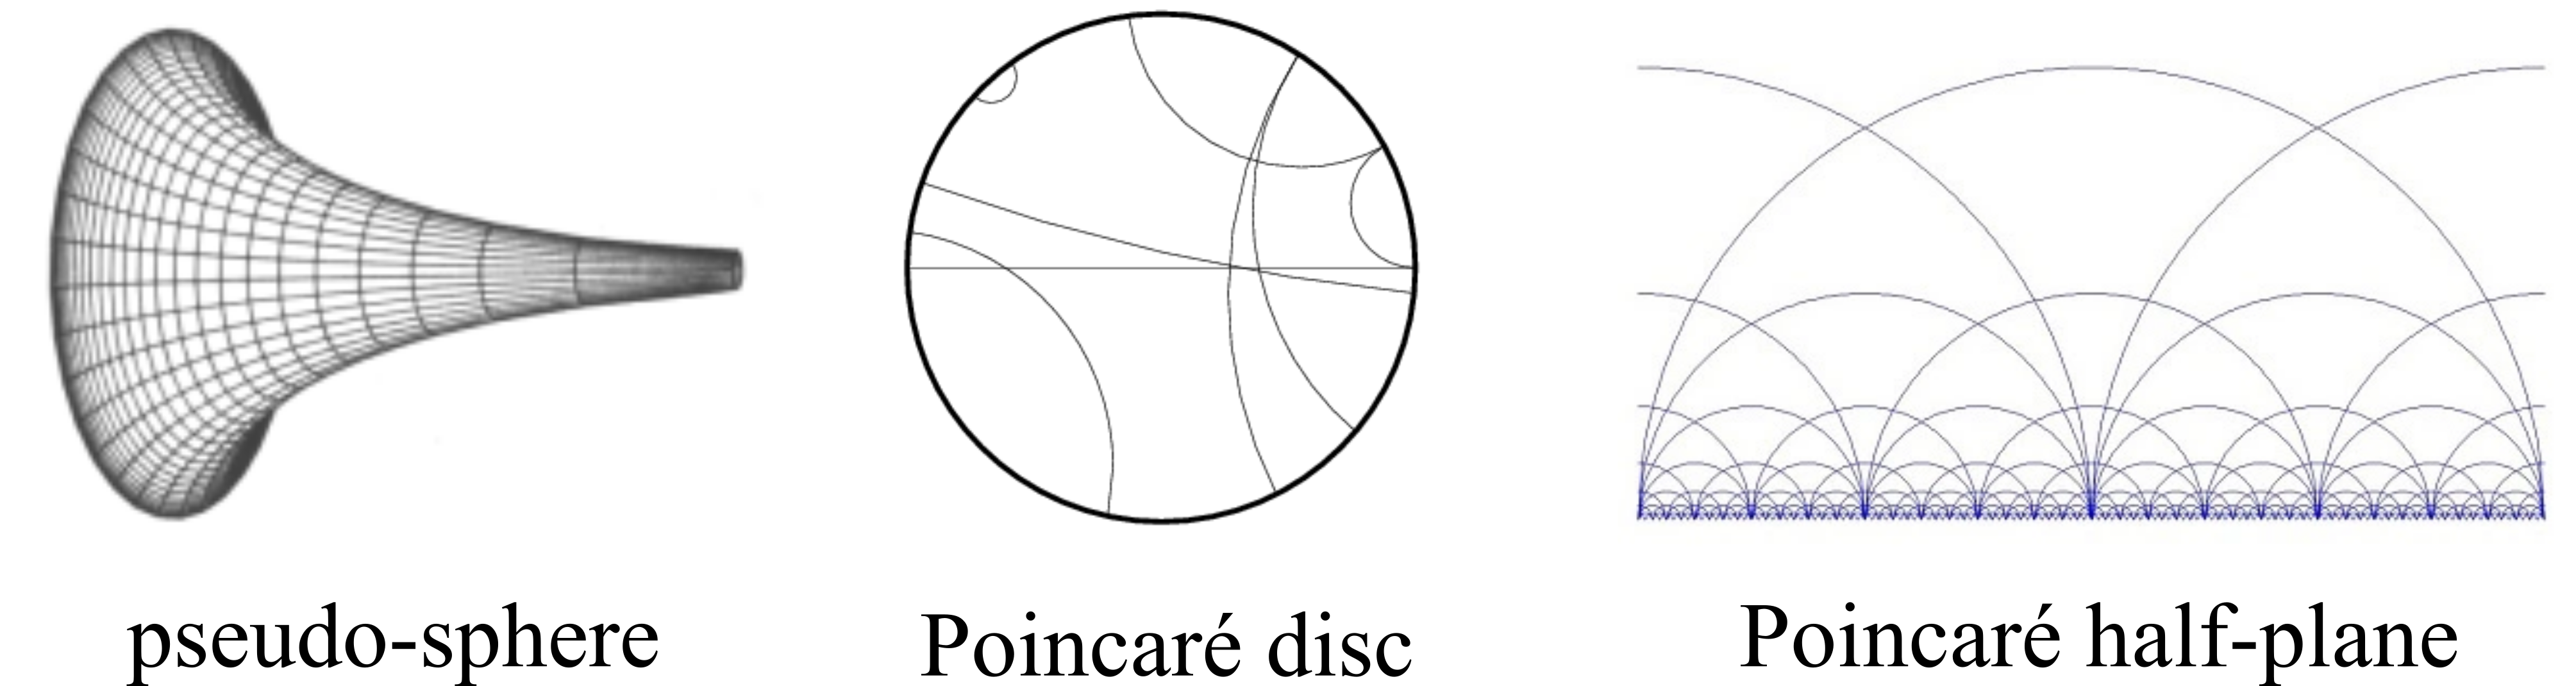
\includegraphics[scale=0.7]{hyperbolic-models.png}}}  \nonumber
\end{equation}
模型不是唯一的,可以有很多种。

在数理逻辑中,\textbf{模型论} 研究的是 syntax / \textbf{theory} 和 \textbf{model} 之间的 \textbf{对偶}。

First-order logic 的 模型 可以用一些 \textbf{集合} 及其 \textbf{元素} 组成。  例如,\\
$\mbox{John} \in \mbox{Male}, \quad \mbox{John, Mary} \in \mbox{Mathematician}$: 
\begin{equation}
\vcenter{\hbox{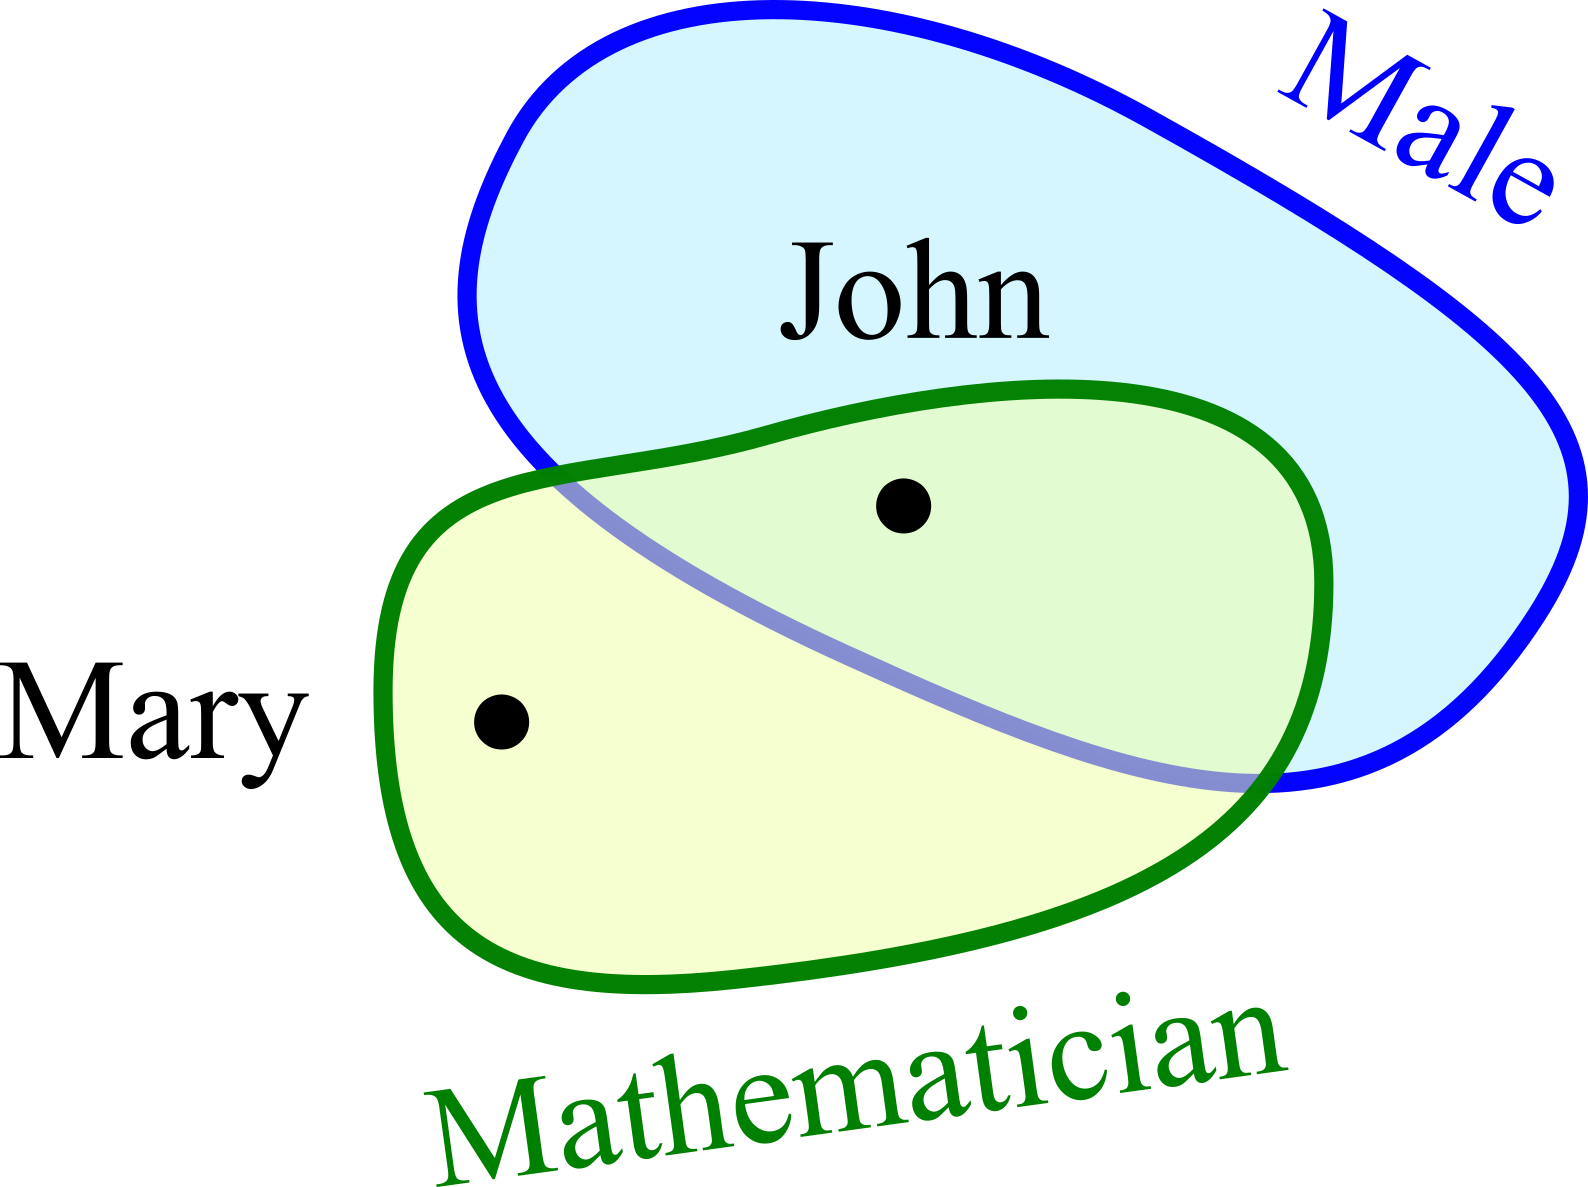
\includegraphics[scale=0.6]{FOL-model-1.png}}} 
\end{equation}
而 first-order objects(\textbf{个体})之间的 \textbf{关系} 是 domain $D$ 的 Cartesian product $D \times D$ 内的一些 \textbf{子集},例如:
\begin{equation}
\vcenter{\hbox{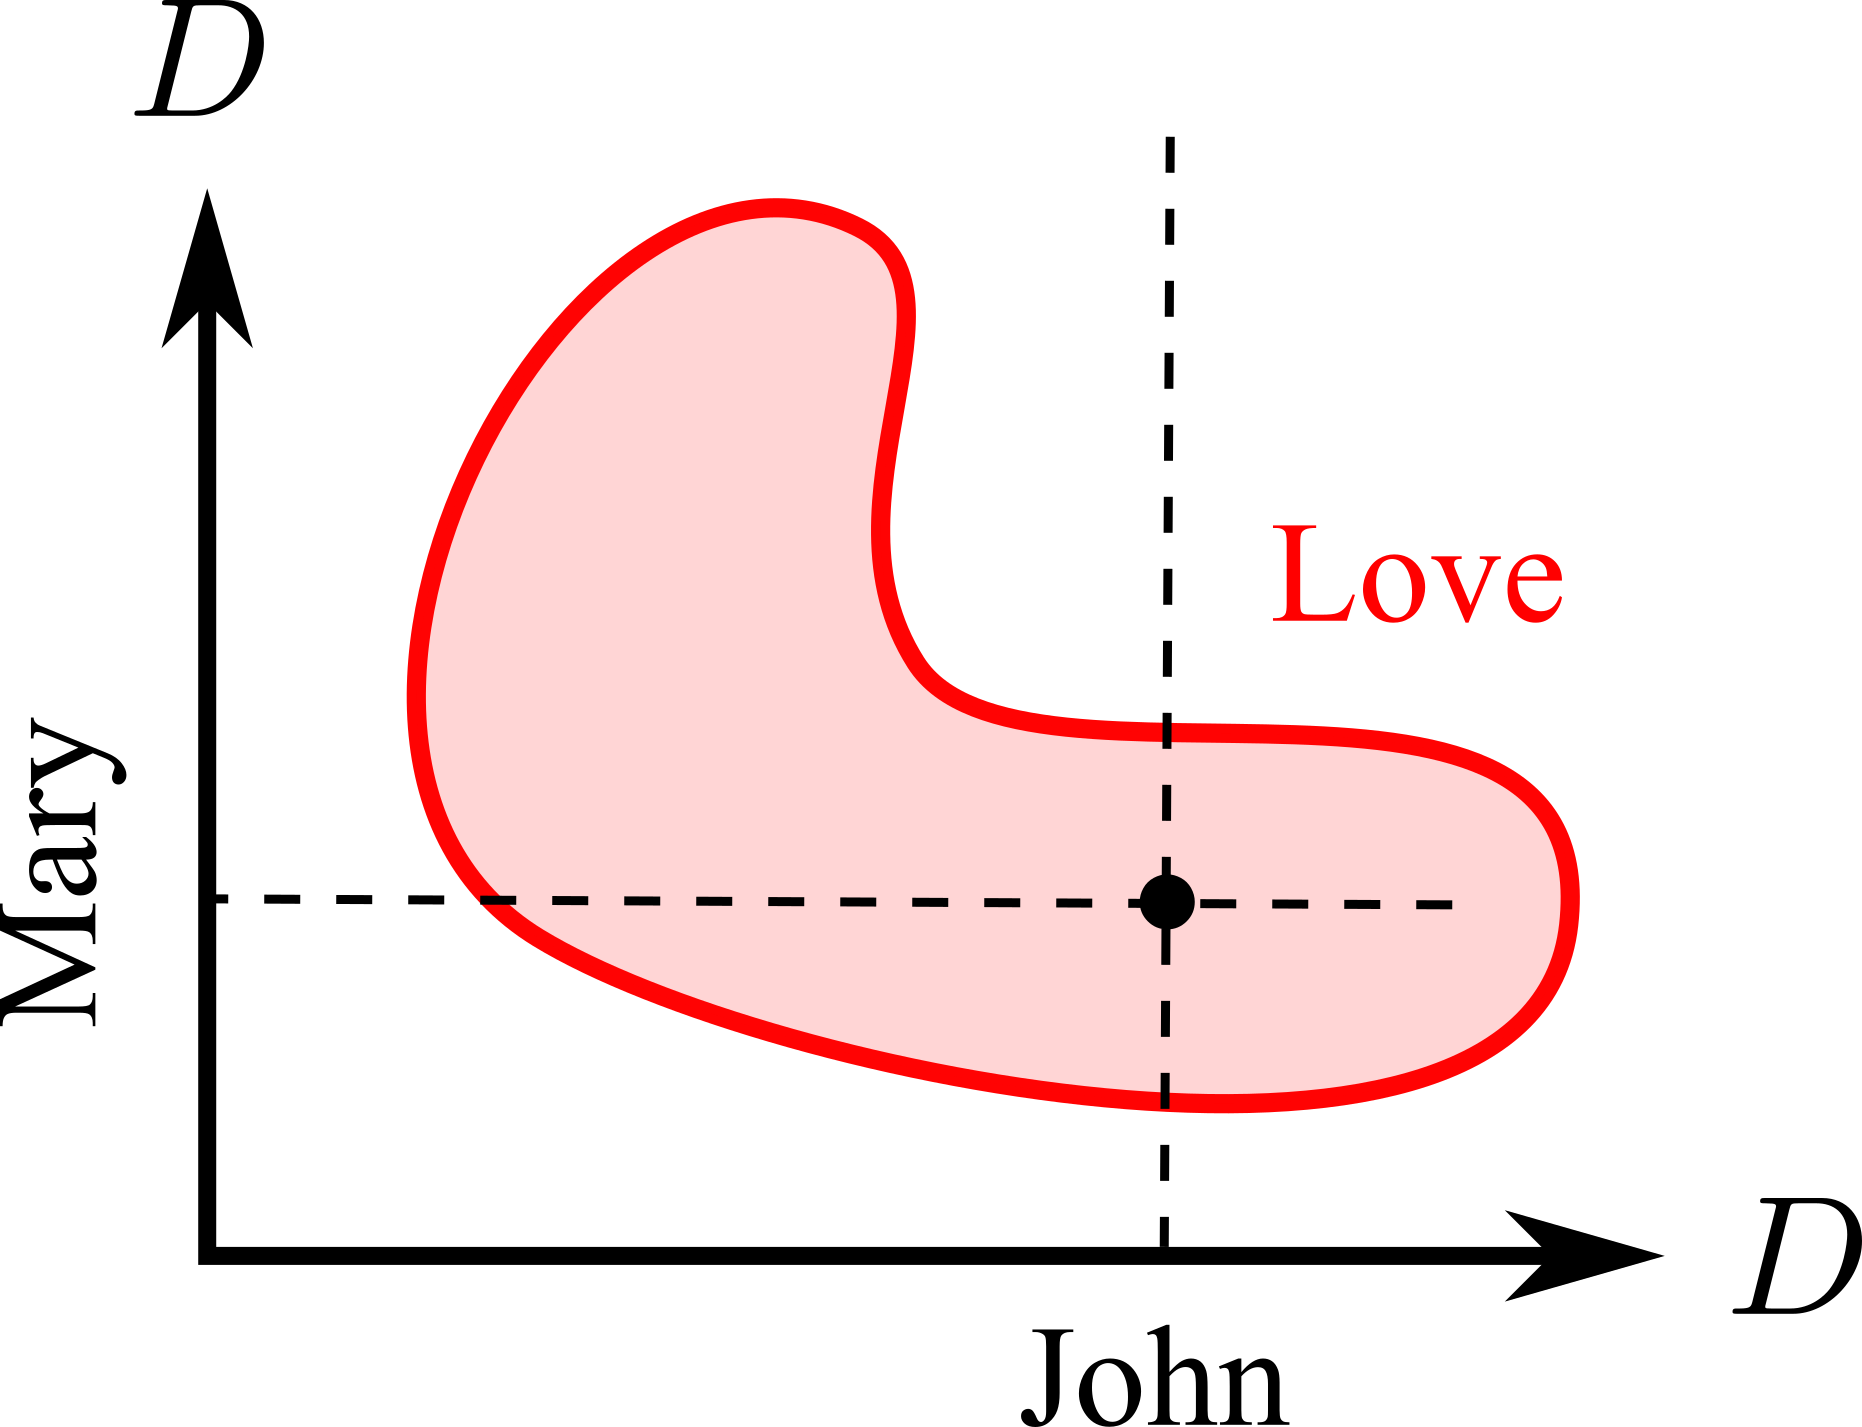
\includegraphics[scale=0.6]{FOL-model-2.png}}} 
\end{equation}

对计算系的人来说,更熟识的 model 是以下这种 relation graph 或 \textbf{knowledge graph}: 
\begin{equation}
\vcenter{\hbox{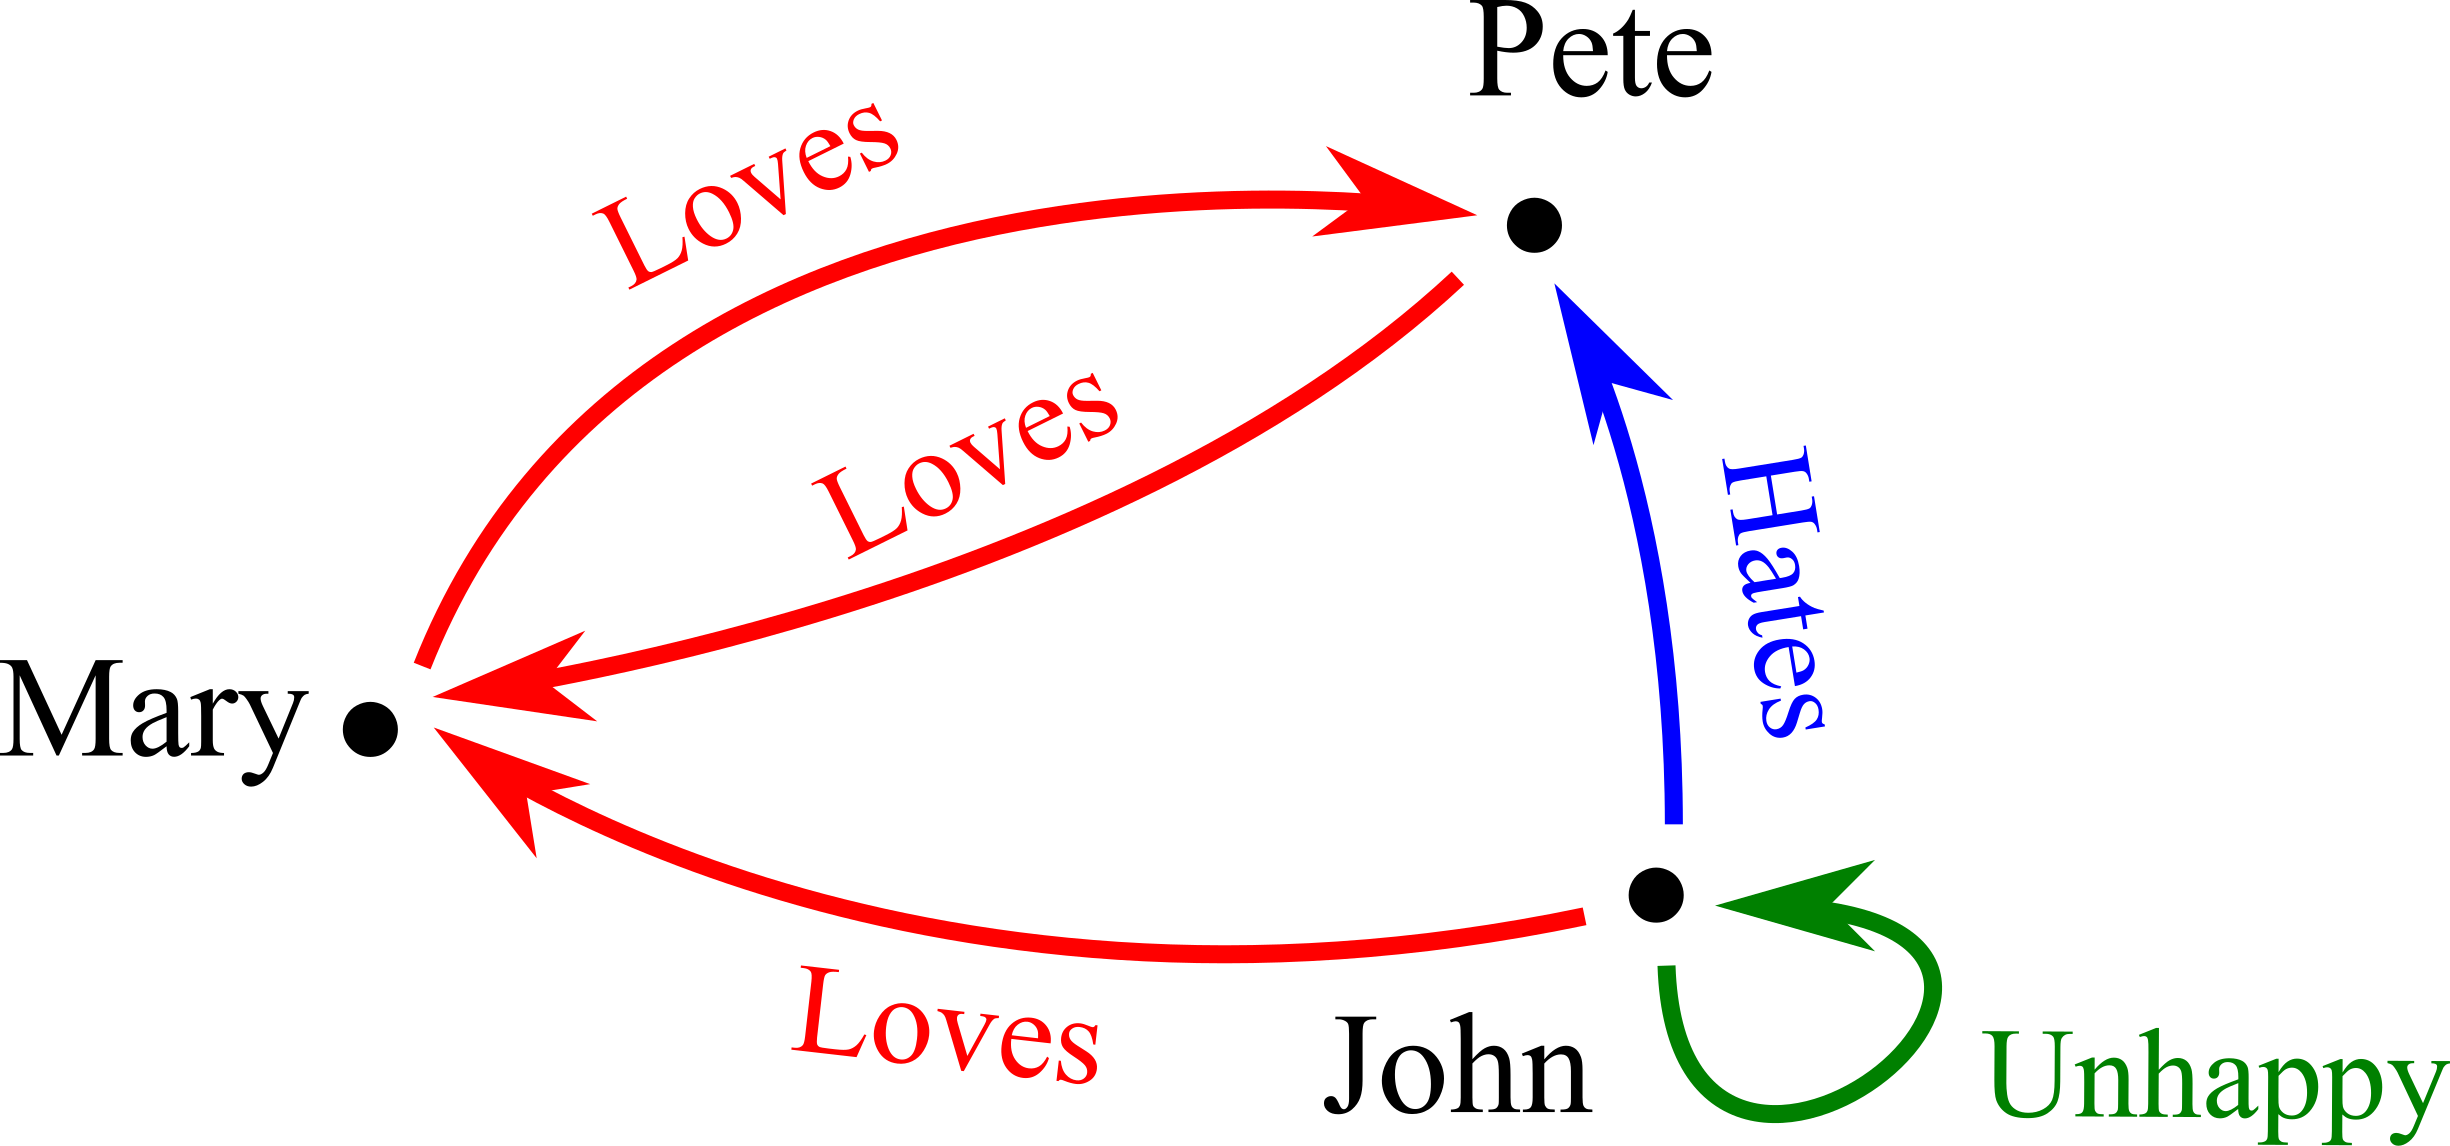
\includegraphics[scale=0.6]{FOL-model-3.png}}} 
\end{equation}
这是一个 \textbf{directed multi-graph},或者叫 \textbf{quiver}。  Quivers 是 代数表示论 (representation theory) 中的重要结构。  Quivers 的范畴 $\mathcal{Q}$ 是一个 \textbf{topos}(这在会 \S\ref{Categorical-semantics} 介绍),基本意思是 \uline{它有条件做 first-order logic 的 }\textbf{\uline{模型}}\uline{范畴}\footnote{根据 \parencite{Grilliette2017} 的说法,hyper-graph 不是 topos,multi-graph 也不是 topos,但当它们变成 directed 则可以。} 。

以上的 knowledge graph 可以简单地转换成 \textbf{逻辑式子} 的集合:
\footnotesize
\begin{equation}
\begin{array}{l}
	\verb|Loves(John, Mary)| \\
	\verb|Loves(Pete, Mary)| \\
	\verb|Loves(Mary, Pete)| \\
	\verb|Hates(John, Pete)| \\
	\verb|Unhappy(John)|
\end{array}
\label{FOL-model}
\end{equation}
\normalsize
所以说,\uline{逻辑 与 graph 基本上是 }\textbf{\uline{等价}}\uline{的}。

\begin{tcolorbox}[breakable, parbox=false]
如果 graph 的每条 边 可以包含任意个 顶点,则有 \textbf{hyper-graph}。 换句话说,hypergraph 的每条 边 $\in \powerset(V)$,$V$ 是 顶点集。 也可以说,hypergraph 就是 V 的 \textbf{子集系统} (set system)。  对逻辑来说,这好处是: \uline{关系 之上可以有 关系}。  

Hypergraph 可以一一对应於拓扑学上的 \textbf{simplicial complex},可以研究它的 homology 和 cohomology。 Simplicial complex 也可以和 \textbf{square-free monomial ideals} 一一对应。 Square-free 的意思是 $x_i$ 的指数只可以是 0 或 1。  后者是 \textbf{组合交换代数} (combinatorial commutative algebra) 的研究范围。  暂时我不知道这些关联有没有用,详细可参看 \parencite{Brown2013}, \parencite{Miller2005}。
\end{tcolorbox}

一个逻辑式子的集合叫 logical \textbf{theory}.  一个代数等式的集合叫 \textbf{algebraic theory}.

例如可以有以下这个逻辑式子(``失恋则不开心''):
\begin{equation}
\forall x,y. \; \mbox{Loves}(x,y) \wedge \neg \mbox{Loves}(y,x) \rightarrow \mbox{Unhappy}(x)
\end{equation}
这个式子含有 universal quantification,所以不是 model 的一部分。 逻辑上来说,只有 \textbf{ground sentences} (没有变量的式子)的集合才可以组成 model,例如 (\ref{FOL-model}) 。 

\section{模型空间 的 fractal 结构}

Logic \textbf{theory} 中的一个式子 可以导致 model 中出现很多 \textbf{新的} 顶点和连接。 这是 model theory 研究的问题。  某些情况下,模型空间 会出现「无限细分」的 fractal 结构。 

例如,每一个自然数 $n \in \mathbb{N}$ 都有 它的 successor $S(n)$。 这个函数的存在,导致 model 空间里有一系列 \textbf{无穷} 的顶点:
\begin{equation}
\textbullet \quad \textbullet \quad \textbullet \quad \textbullet \quad \textbullet \quad \textbullet \quad \textbullet \quad \textbullet \quad \textbullet \; .....
\end{equation}
如果加入这条 \textbf{法则}:
\begin{equation}
\forall n \in \mathbb{N}. \quad S(n) \ge n
\end{equation}
则立即产生无穷多个关系:
\begin{equation}
\textbullet \stackrel{\ge}{\longleftarrow} \textbullet \stackrel{\ge}{\longleftarrow} \textbullet \stackrel{\ge}{\longleftarrow} \textbullet \stackrel{\ge}{\longleftarrow} \textbullet \stackrel{\ge}{\longleftarrow} \textbullet \stackrel{\ge}{\longleftarrow} \textbullet \stackrel{\ge}{\longleftarrow} \textbullet \; .....
\end{equation}
虽然,在 \textbf{日常智能} (common-sense intelligence) 中,似乎比较少出现这种无穷的结构,而更多是 ``shallow'' 的结构。 

\footnotesize
附带一提,经典逻辑人工智能 (classical logic-based AI) 的知识表述 是分拆成 \textbf{rules} 和 \textbf{facts} 两部分。 前者是带有 $\forall$ \textbf{变量} 的式子,后者是 ground sentences。  Rules 储存在 $\KB$ 内,facts 储存在 \textbf{working memory} 内。 前者是一个 \textbf{theory},后者可以看成是一些 \textbf{``partial'' models}。  说 partial 的原因是因为它不代表整个 model。  事实上 model 是非常庞大的东西,不可能储存在物理系统中。  人工智能或大脑只能储存 某些 theories 和部分的 models。  人工智能的关键问题是如何找一种良好的 syntax 结构,令 theory 的学习更快、更有效率。 
\normalsize

\section{强人工智能的简单表述}

这一节用尽量简练的方式描述强人工智能系统的数学结构,即使没有 AI 背景的数学家也能看懂。

\begin{tcolorbox}[breakable, parbox=false]
重温一下 \textbf{神经网络} 是这样的:
\begin{eqnarray}
\mbox{\footnotesize 每层的} \tikzmark{ww} \mbox{\footnotesize \textbf{权重}矩阵} \quad \quad \mbox{\footnotesize 总层数} \tikzmark{LL} \nonumber \\
\nonumber \\
F(\vec{x}) = \sigmoid(W_1 \tikzmark{wa} \sigmoid(W_2 \tikzmark{wb} ... \sigmoid( W_L \tikzmark{wc} \tikzmark{L} \; \vec{x} )))
\begin{tikzpicture}[overlay,remember picture]
  \draw[-, shorten <=12pt, transform canvas={shift={(-10pt,10pt)}}] (ww.center) to (wa.center);
  \draw[-, shorten <=16pt, transform canvas={shift={(-10pt,10pt)}}] (ww.center) to (wb.center);
  \draw[-, shorten <=28pt, transform canvas={shift={(-10pt,10pt)}}] (ww.center) to (wc.center);
  \draw (LL.center) +(-15pt,-3pt) -- ([shift={(-2pt,6pt)}]L.center);
\end{tikzpicture}
\end{eqnarray}
它的 \textbf{参数} 集合 $\Theta = \{ W_{i, j}^{\ell} \} \in \mathbb{R}^m$,其中 $m$ = \# weights。 

\textbf{机器学习} 的目的是 \uline{寻找 optimal $\Theta$ subject to an objective function}.  换句话说,机器学习 = \textbf{optimization},这是应用数学的最基本问题之一。

训练时,给定一组 data points($F$ 是神经网络):
\begin{equation}
\label{NN-training}
\boxed{\mbox{training examples}} \quad
e \stackrel{F}{\longrightarrow} a
\quad \boxed{\mbox{answers}} 
\end{equation}
每个答案的误差是 $\epsilon$,目标函数 $J$ 是很多次 iterations 的误差之和。
% \begin{equation}
% J = \sum_t \epsilon \; ( e, a, \Theta )
% \end{equation}
我们想令 $J$ 最优化,方法是计算 $J$ 对于 $\Theta$ 的梯度 (gradient):
\begin{equation}
\nabla_{\Theta} J := \frac{\partial J}{\partial \Theta}
\end{equation}
当然这就是著名的 back-propagation 算法,其实即 gradient descent。
\end{tcolorbox}

\begin{tcolorbox}[ams equation, colback=yellow, colframe=white]
\mbox{强人工智能 的樽颈问题 是\textbf{学习算法}的速度}
\end{tcolorbox}

AI 学习算法的特点是 \uline{需要在 }\textbf{\uline{ 逻辑式子}}\uline{ 上进行最优化}:
\begin{tcolorbox}[ams align, colback=yellow, colframe=white]
\mbox{从 } \mbox{ optimization over $\mathbb{R}$} && \mbox{ 过渡到 } & \mbox{ optimization over $\mathcal{L}$} \nonumber\\
\Theta \in \mathbb{R}^m && \rightsquigarrow & \; \; \Theta \in \mathcal{L}
\end{tcolorbox}
其中 $\mathcal{L}$ 是某种 (例如一阶谓词)\textbf{逻辑语法},$\Theta$ 是一个逻辑式子的集合。 这最优化问题的解 $\Theta^*$ 是一个 optimal logic theory。

系统的 top-level architecture 是 强化学习,亦即 dynamic programming,是 optimization 的一个特例,也可以叫 control theory,它控制的\textbf{系统}是:
\begin{equation}
\vec{x}_{n+1} = \vec{f}( \vec{x}_n, \vec{u}_n )
\end{equation}
$\vec{x}$ 是系统的\textbf{状态},$\vec{u}$ 叫 control 或 action。 在 AI 里,$\vec{x}$ 是「思维空间」中的\textbf{位置},$\vec{u}$ 是「思考」的 steps。 我们希望控制 $\vec{u}$,令系统在\uline{长时间的运行中},收到的\textbf{奖励}达到最大值: 
\begin{equation}
\boxed{\mbox{total rewards}} \quad J = \sum_n L(\vec{x}) = \int L dt
\end{equation}
$L \in \mathbb{R}$ 是在 $\vec{x}$ 位置得到的\textbf{瞬时奖励},基於历史上分析力学的原因,$L$ 也叫作 \textbf{Lagrangian},单位是能量,但注意这里的 $\vec{x}$ 是「思维空间」,不同於物理空间。 我附带写上微分形式,以便於记忆。

系统的运行如下:
\begin{equation}
\vcenter{\hbox{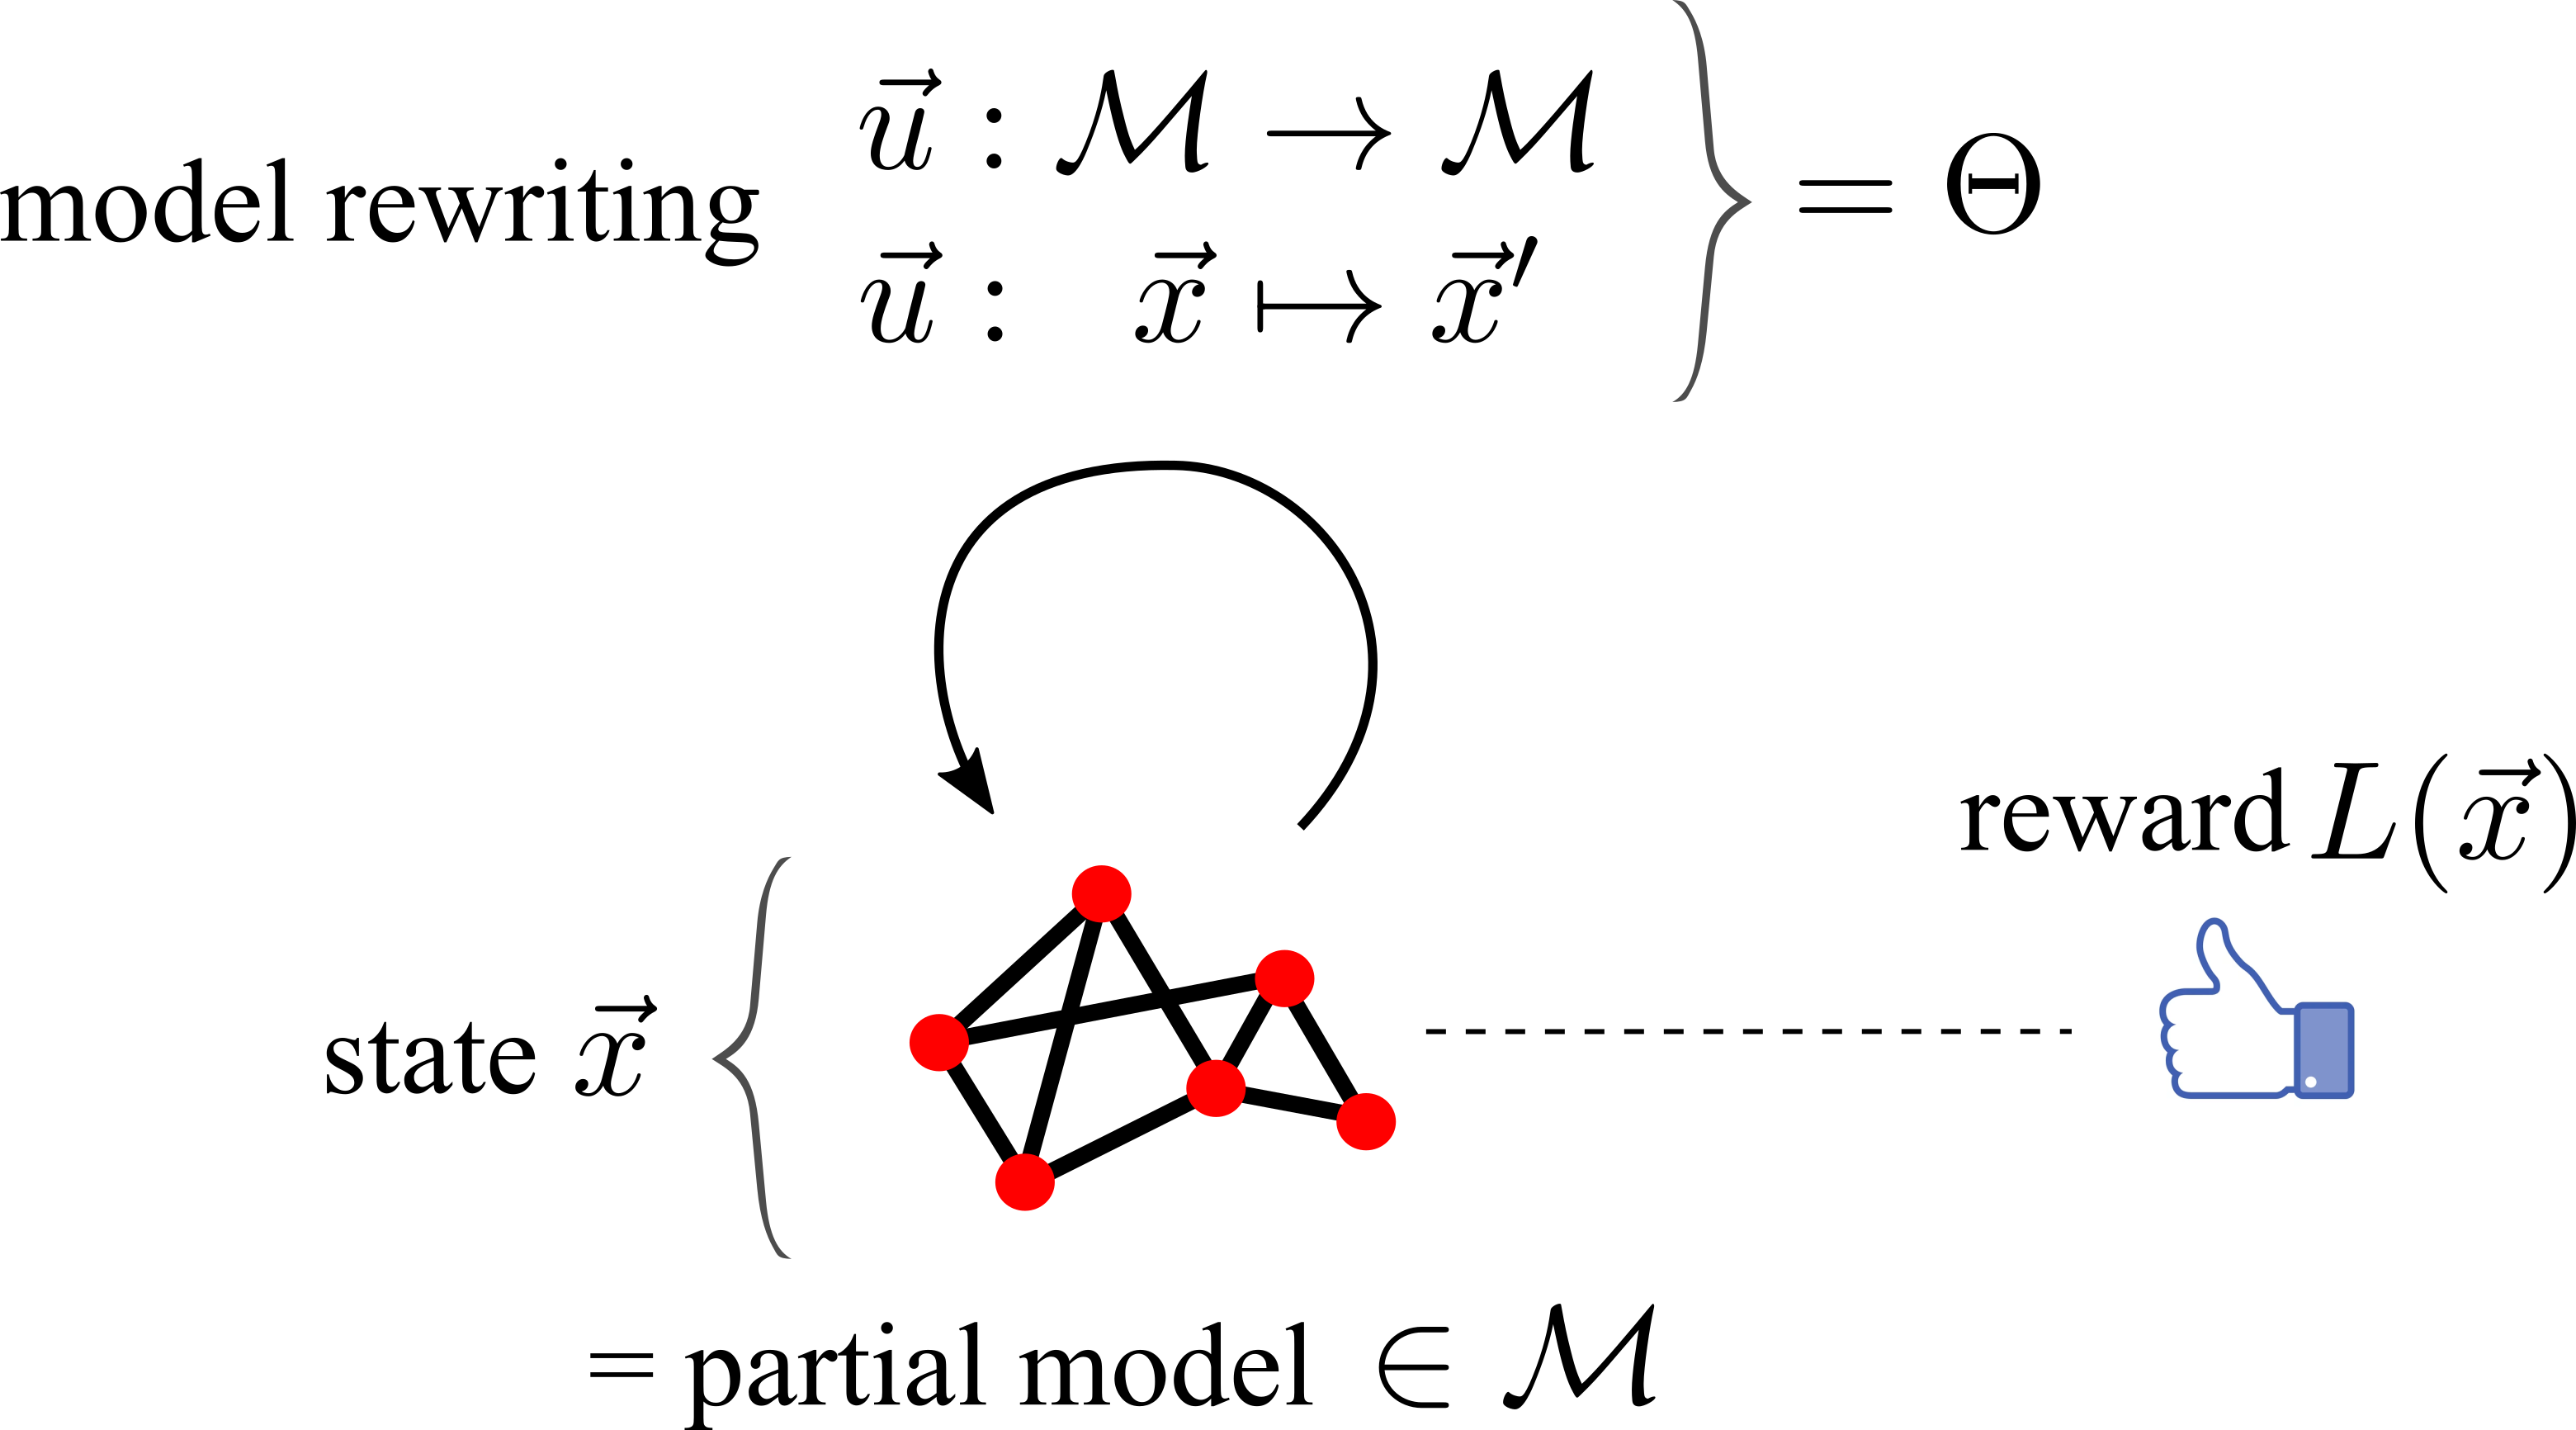
\includegraphics[scale=0.7]{abstract-dynamic-programming.png}}}
\end{equation}
% $\vec{x}$ 的某些部分用作\textbf{输出},经由它得到奖励。 
$\vec{u}$ 和 $\vec{f}$ 重合,作用是将 $\vec{x}$ \textbf{重写}。 Optimization 作用在 $\Theta$(亦即 $\vec{u}$)之上。  注意 $\vec{u} \in$ 某种 function space,例如是一些 逻辑式子,这和传统的 optimization over $\mathbb{R}$ 很不同。 

\footnotesize
在经典 AI 中,$\vec{u}(\vec{x}) = \vec{f}(\vec{x})$ 的作用相当於 deduction $\vec{x} \vdash \vec{x}'$,或者叫 forward-chaining(向前推导出一些逻辑结论)。  在经典 AI 中这工作由 \textbf{逻辑引擎} 负责,它包含 \textbf{unification} (= rule matching) 和 \textbf{resolution} (= proof search) 两个算法。  在我们的框架中 看不到这些运作,因为它们被包含在 $\vec{u}$ 或 $\vec{f}$ 之内。 
\normalsize

%训练的过程类似 (\ref{NN-training}):
%\begin{equation}
%\boxed{\mbox{training examples}} \quad
%e \sststile{}{\Theta} a
%\quad \boxed{\mbox{answers}} 
%\end{equation}
%但现在 $\vdash$ 是根据 $\Theta$ 的 \textbf{逻辑推导},$e$ 和 $a$ 是逻辑式子的集合。 给定一些前提,可以推出很多结论,其中有些得到奖励或惩罚。 % 在 \textbf{强化学习} (reinforcement learning,亦即 dynamtic programming) 的框架下,训练是根据 \textbf{奖励} 而不是 \textbf{误差},和上面略有不同。 

分析力学中 Hamiltonian 的定义是:
\begin{equation}
H = L + \frac{\partial J}{\partial \vec{x}} \vec{f}
\end{equation}
类似地,\textbf{离散}系统的 Hamiltonian 可以定义为:
\begin{equation}
H = L + J ( \vec{f}(\vec{x}) )
\end{equation}
Pontryagin\footnote{Lev Pontryagin (1908-1988) Soviet mathematician. Blind since the age of 14, he made major discoveries in a number of fields including algebraic topology and differential topology.} 的 \textbf{极小值原理} 给出最优解的条件是:
\begin{equation}
H^* = \inf_u H
\end{equation}
可以定义一个作用在 J 上的算子 T:
\begin{equation}
T J := \inf_u H
\end{equation}
则 Bellman's optimality condition 可以表示为以下的 fixed-point 形式:
\begin{equation}
J^* = T J^*
\end{equation}
相信应用数学方面的专家们比我更熟悉这些理论..... 据说 Hamilton-Jacobi 方法导致解 偏微分方程,不是特别有效,实践中更有用的是 Pontryagin 极小值原理。 

关键是: $\Theta$ 属於的 domain 不是传统的 $\mathbb{R}^n$。 如果想用传统的 基於 differentials 的 optimization 技巧,似乎最低要求是 domain 上的 topology、continuity 和 compactness,然后才可以定义例如 Fr\'{e}chet derivative.

\section{Plan 0: geometric models}

\begin{tcolorbox}[ams equation, colback=yellow, colframe=white]
\mbox{一阶逻辑语法 $\mathcal{L}$ 不是必需的,只需某种将 model \textbf{改写} 的能力}
%\uline{一阶逻辑语法 $\mathcal{L}$ 不是必需的,只需要某种将 model }\textbf{\uline{改写}}\uline{的能力}。 
\end{tcolorbox}
可以有很多不同的变种,例如:
\begin{equation}
\begin{tikzcd}[column sep = large]
\mbox{逻辑语法 } \; \mathcal{L} \arrow[d] \\
\mbox{partial model } \mathcal{M}
\end{tikzcd}
\approx
\begin{tikzcd}[column sep = large]
\mbox{graph re-writer} \arrow[d] \\
\mbox{graph model}
\end{tikzcd}
\end{equation}

考虑一种我称为 \textbf{geometric model} 的模型,例如:
\begin{equation}
P(x) \wedge Q(x) \quad \cong \quad
\vcenter{\hbox{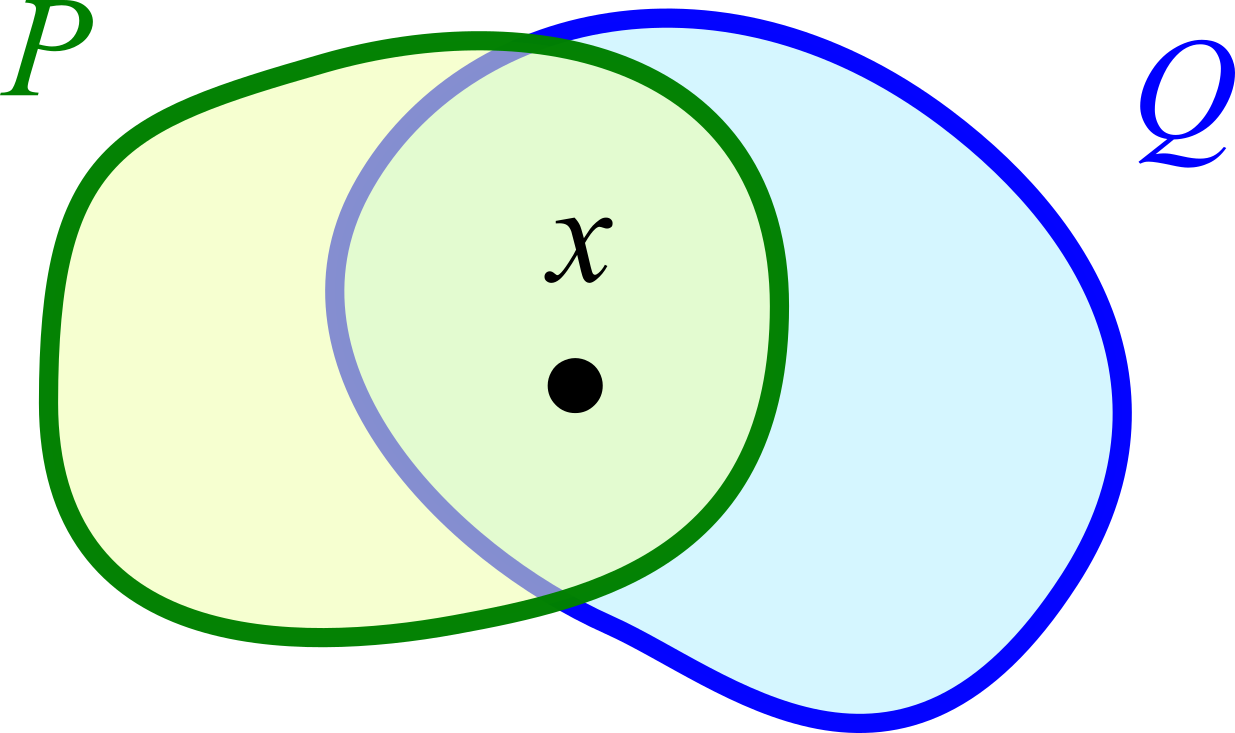
\includegraphics[scale=0.7]{Venn-diagram.png}}}
\end{equation}
这是大家熟悉的 Venn diagram,也是 \textbf{Stone duality} 的最经典例子。 Stone\footnote{Marshall Stone (1903-1989), American mathematician who contributed to real analysis, functional analysis, topology and the study of Boolean algebras.} duality 指的是 Boolean algebra 和 topological space 之间的对应。  

这些 geometric ``\textbf{regions}'' 很容易用神经网络做到。 如果 $\vec{F} =$ 神经网络,则:
\begin{equation}
\vec{F}(\vec{x}) = 0
\end{equation}
定义了一个 hyper-surface of co-dimension 1,它将周围的空间分割为 $> 0$ 和 $< 0$ 两部份。 

希望做到(但或许很难做到)的一个效果是: \uline{一个逻辑式子能连续地 deform 成另一个不同的式子}。 在经典逻辑中这是不可能的,例如 $\mbox{Love}(x,y)$ 和 $\mbox{Like}(x,y)$,虽然意思接近,但从一个变成另一个必需 discrete 的跳跃。 如下图,两个近似的 regions :
\begin{equation}
\vcenter{\hbox{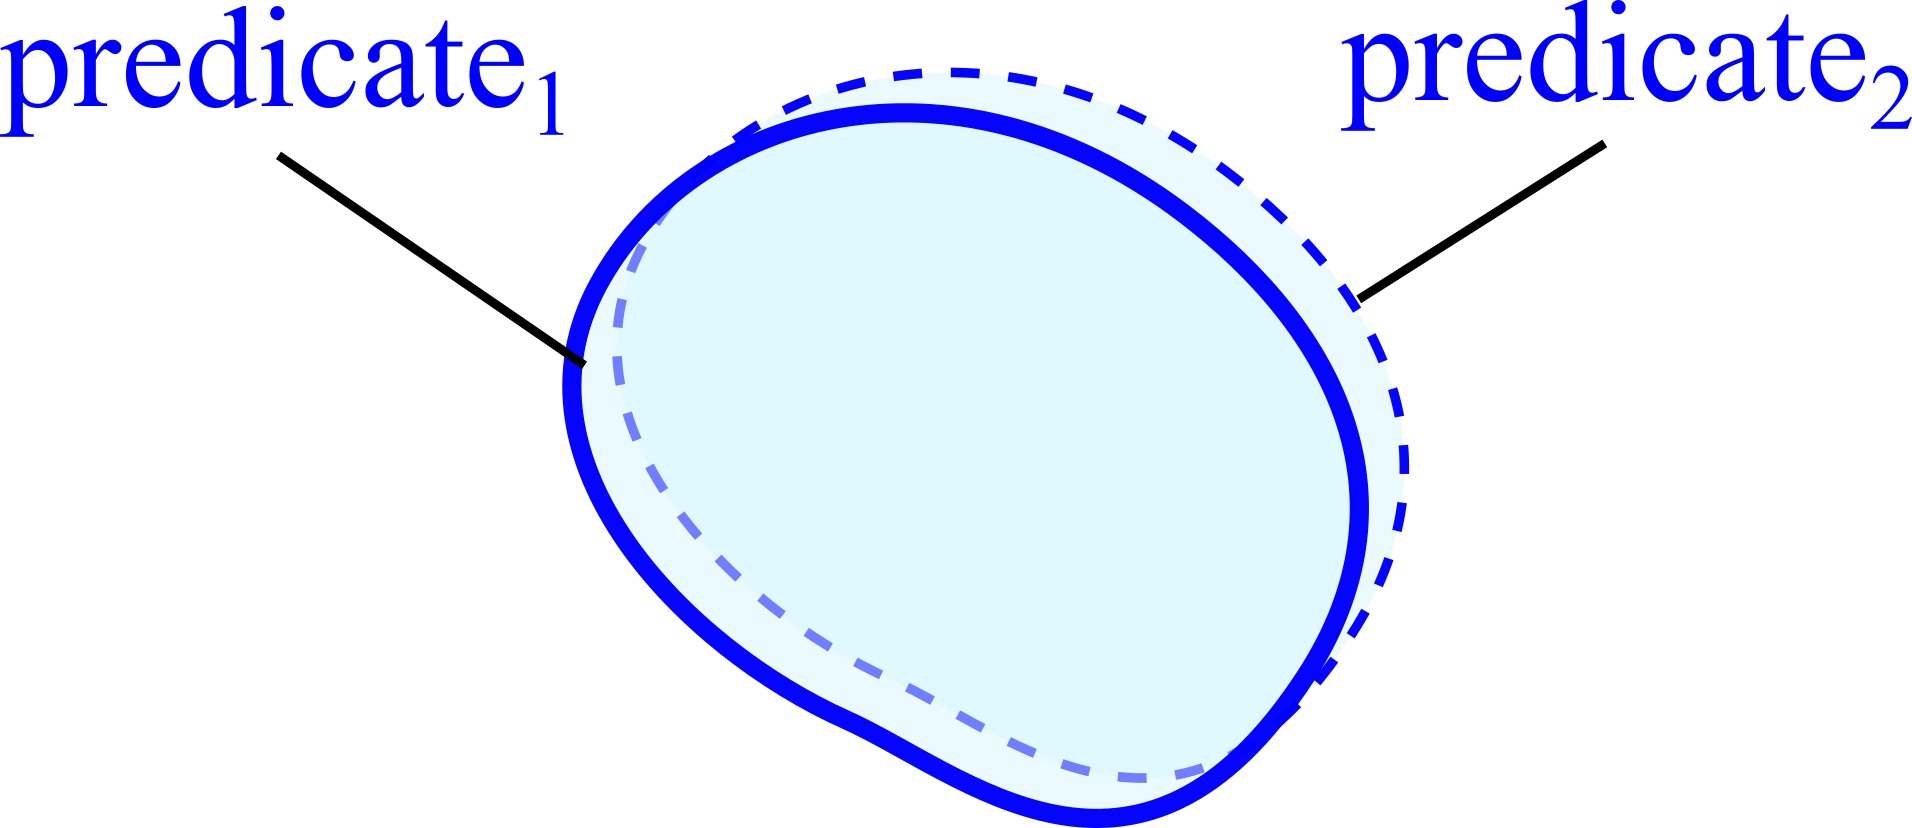
\includegraphics[scale=0.7]{nearby-predicates.png}}}
\end{equation}
它们是不是两个 distinct objects 视乎 representation 怎样而决定。

% 根据 范畴论 的看法,一个集合里的\textbf{元素},是一个 $\mathbf{1} \rightarrow \mathbf{Set}$ 的 mapping。  如果我们不想要「一粒粒」的元素,或许可以用 $\mathbb{R} \rightarrow \mathbf{Set}$ 这样的 mapping? 

总括来说,这个方案是:
\begin{eqnarray}
\mbox{model } \mathcal{M} &=& \mbox{geometric models of set theory} \nonumber \\
\mbox{rewriter} &=& \mbox{functor } \mathcal{M} \rightarrow \mathcal{M}
\end{eqnarray}
但我们需要一个 \uline{可以连续变化的} model of set theory,或许可以用某种 fuzzy topology 来达成?  这是我未来会专注的方向。

% 当然,如果改写的能力太弱,则会 ``throw the baby out with the water'',亦即丧失了一阶逻辑的\textbf{泛化}能力。  同时,要从 optimization 的角度考虑,什么形式的改写才最有利於速度。  模型的 representation 也是一个考虑因素: 它应该有某种良好的 \textbf{metric},这 metric 近似 semantic distance,而不是纯粹基於 logic syntax。 事实上,完美的 semantic metric 是\textbf{不可计算的},因它是 Kolmogorov complexity.

以下主要分析 plan A 和 B(它们已经是可行的)。

\section{Plan A: genetic algorithm}
\label{COCO}

\begin{tcolorbox}[ams equation, colback=yellow, colframe=white]
\mbox{放弃梯度下降}
\end{tcolorbox}
\begin{eqnarray}
\mbox{model } \mathcal{M} &=& \mbox{符号逻辑式子} \nonumber \\
\mbox{rewriter} &=& \mbox{符号逻辑式子 + 经典 AI 逻辑引擎}
\end{eqnarray}

GA 本来就非常适合\textbf{离散}的搜寻空间,它和逻辑结构很兼容,在这条路线上已经没有理论上的 obstructions. 

% \section{Plan A: 协同进化 (COCO)}

% Substitution 的麻烦令我想到 \uline{放弃用 neural network 直接处理逻辑,而是用 hybrid 的 神经/逻辑 混合}: 视觉神经用 deep neural network,到高层次转用符号逻辑表述,后者用 genetic algorithm 做学习。

首先需要一个 logic-based \textbf{rule engine},它负责 forward-chaining(正向逻辑推导),这完全是经典 AI 的范围。 例如 经典的 Soar architecture [Carnegie-Mellon 大学] 就是一个 rule-base 引擎。 % 还有我这一代的 OpenCog, OpenNARS, 和我写的 Genifer\footnote{Genifer 仍未到达 production stage.},或许还有更新一代的 AGI 系统(?)  

% 经典逻辑 AI 的樽颈问题是 \uline{rules 的学习算法太慢},
%\begin{itemize}
%\item plan A: 继续用经典逻辑引擎,用 genetic algorithm 做学习算法
%\item plan B: 将逻辑记忆映射到向量空间,再用神经网络学习逻辑 rules
%\end{itemize}

基因算法的 population 是由个别的逻辑 rules 组成,但 winner 并不是单一条 rule,而是一整套 rules(最高分的 $N$ 个)。 这叫 \textbf{cooperative co-evolution}(COCO)。  

输入和输出是 logic formulas,其实更易处理。 

整个系统仍然是基於 reinforcement learning 的,但不需要直接做 RL,因为那些 rules 其实就是 \textbf{actions},每条 rule  的 probabilistic strength 就像 $Q$-learning 中 $Q$值的作用。 

[ 我还未有时间 survey COCO 的实践理论。 ]

\section{Plan B: neural network / deep learning}

馀下大部份篇幅都是为了解决如何用 NN 实现 经典逻辑引擎 的问题,特别是 variable substitution 的问题,最后发觉问题的癥结在於缺少了 short-term memory 的机制。

解决办法是 用 graph 做\textbf{记忆系统},用神经网络做 graph re-writing,亦即 Google / DeepMind 提出的 graph neural network,这是一种 ``hybrid'' architecture.

\subsection{神经网络 处理 substitutions 的困难}
\label{NN}

考虑上节讲过的 逻辑 rule(``失恋则不开心''):
\begin{equation}
\forall x,y. \; x \heartsuit y \wedge \neg y \heartsuit x \rightarrow \frownie{} x
\end{equation}
这个 rule 的 \textbf{前件} (antecedent) 要成立,必须 \uline{两次出现的 $a$ }\textbf{\uline{相等}}\uline{、两次出现的 $b$ }\textbf{\uline{相等}}:
\begin{equation}
\vcenter{\hbox{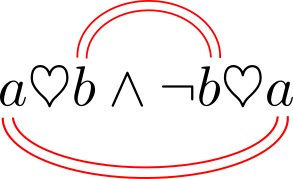
\includegraphics[scale=0.6]{antecedents-equal.png}}}
\end{equation}
而且,要产生正确的 \textbf{后件} (consequent),需要从前件中将 $a$ \textbf{copy} 过来:
\begin{equation}
\vcenter{\hbox{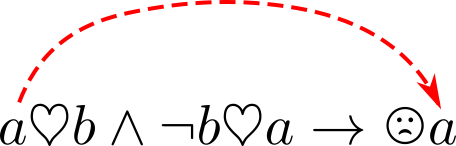
\includegraphics[scale=0.6]{consequent-copy.png}}}
\end{equation}
\uline{这两个动作(\textbf{compare} 和 \textbf{copy})都是用神经网络 很难做到的}。  但它们是 variable substitution 的本质,也是 谓词逻辑 麻烦之处。 换句话说,很难用一个 monolithic 的 end-to-end 神经网络 一口气完成这两个动作:
\begin{equation}
\vcenter{\hbox{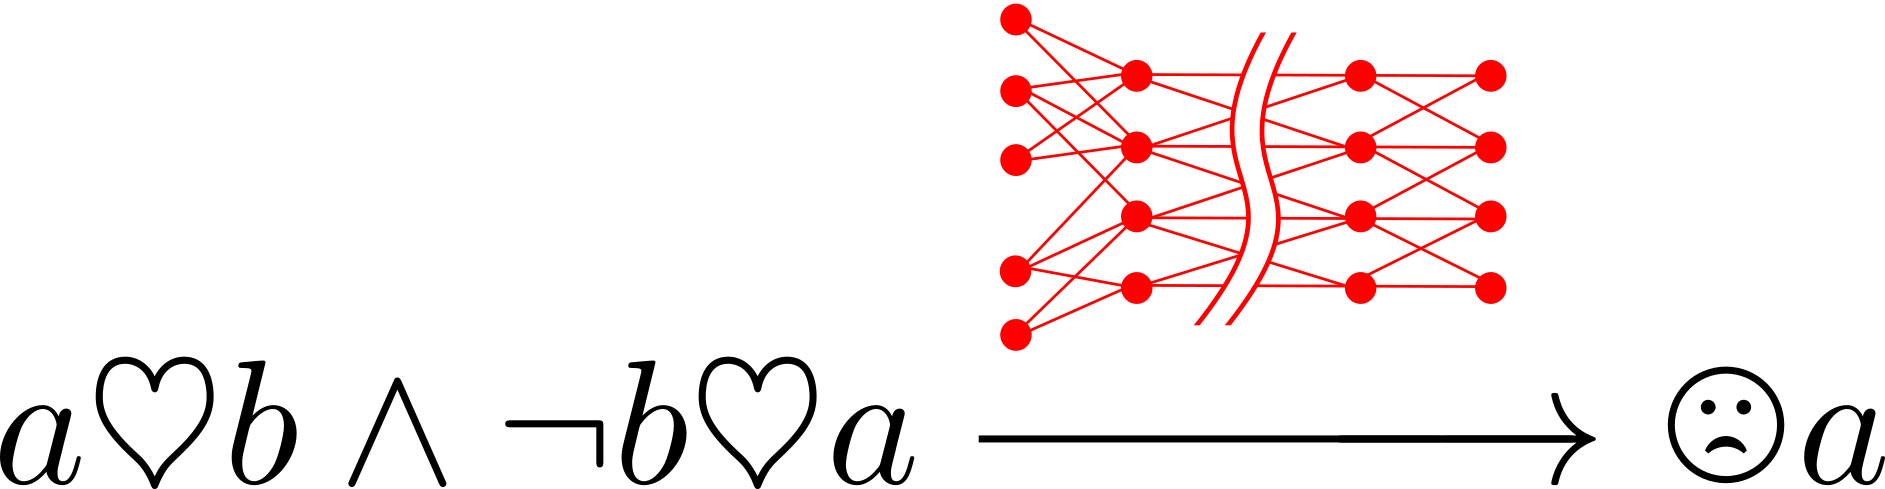
\includegraphics[scale=0.6]{monolithic-NN.png}}}
\end{equation}

首先考虑\textbf{后件}的 copy 问题。 为简单起见,假设逻辑 variable $z$ 对应於 输入向量 $\vec{x}$ 中的某些分量,例如 $x_i$.  Copy 的作用是将 $x_i$ 抄到 $y_j$ 的位置:
\vspace*{10pt}
\begin{equation}
\vec{F}: \; (x_1, ..., {\color{red} x_i} \tikzmark{a}, ... , x_n) \mapsto (y_1, ... , \tikzmark{b} {\color{red} y_j} , ... , y_n)
\begin{tikzpicture}[overlay,remember picture,out=45,in=135,distance=1.1cm]
  \draw[->,red,shorten >=7pt,shorten <=7pt] (a.center) to node [auto, above=2pt] {$id$} (b.center);
\end{tikzpicture}
\end{equation}
这要求神经网络的函数曲面穿过某些 diagonal 线,如下图:
\begin{equation}
\vcenter{\hbox{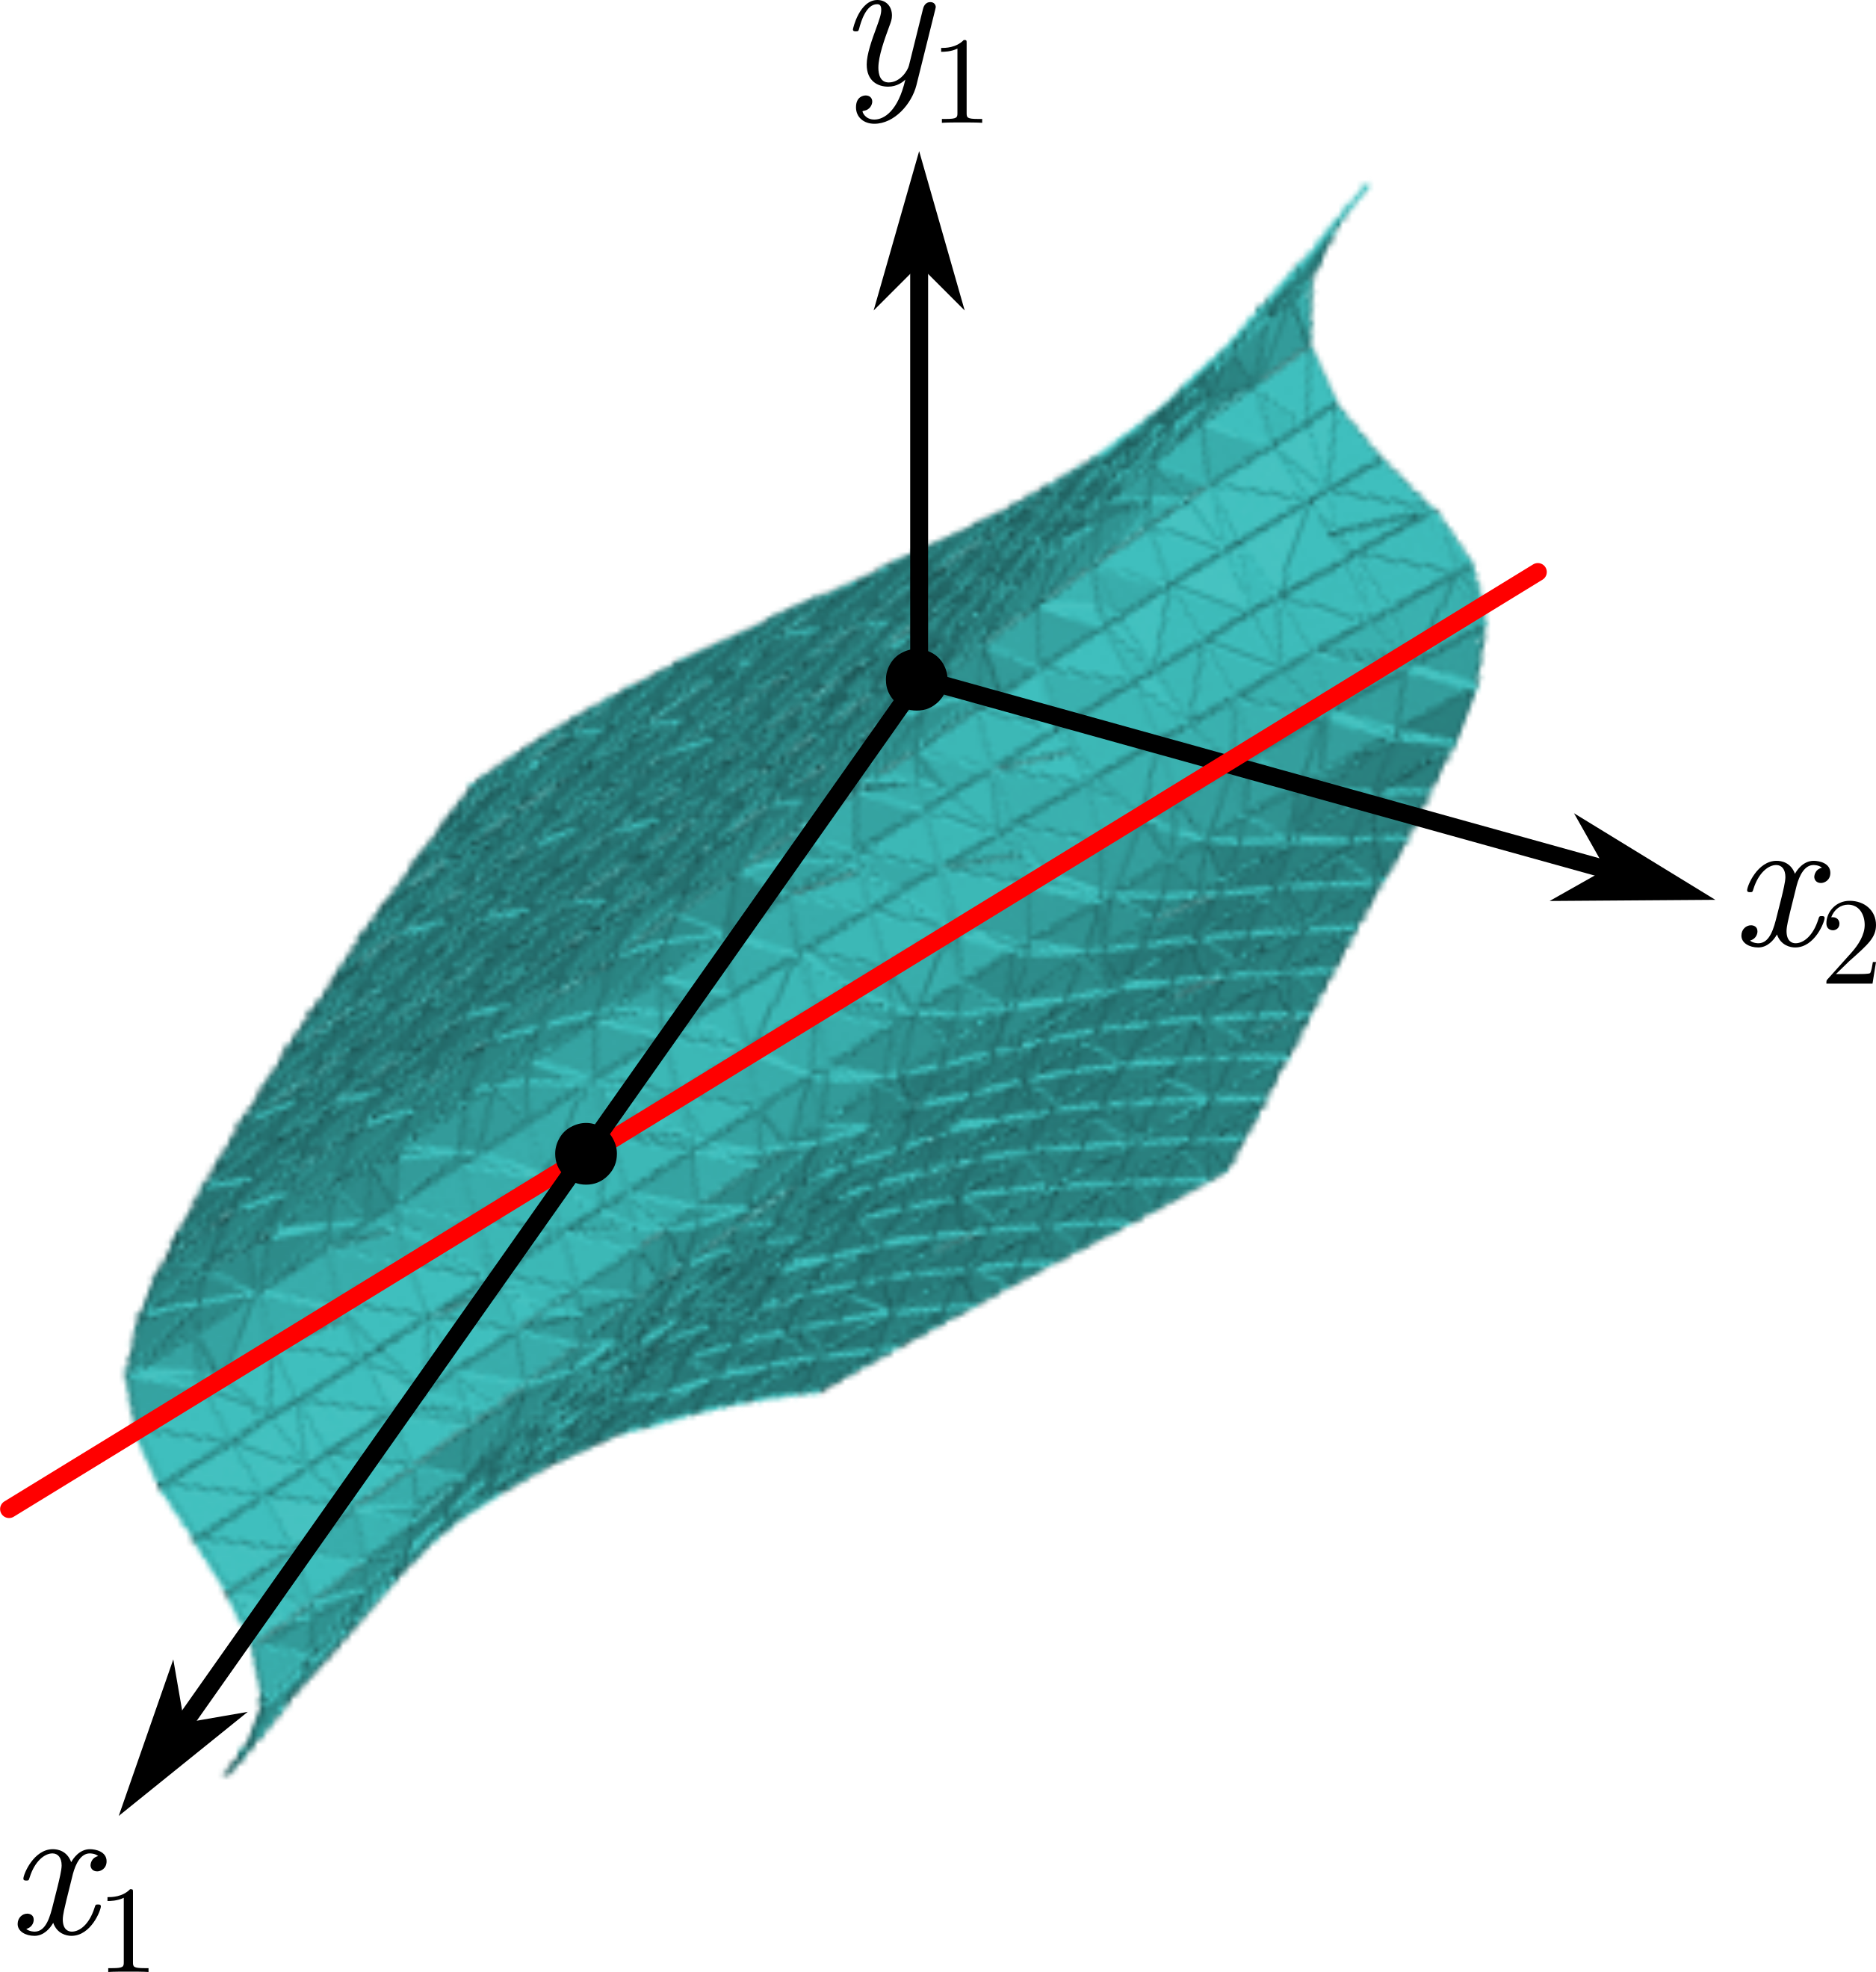
\includegraphics[scale=0.4]{diagonal.png}}}
\end{equation}
以下是一个简单的 copier 神经网络(所有权重 = 1,其他权重 = 0 没有显示):
\begin{equation}
\vcenter{\hbox{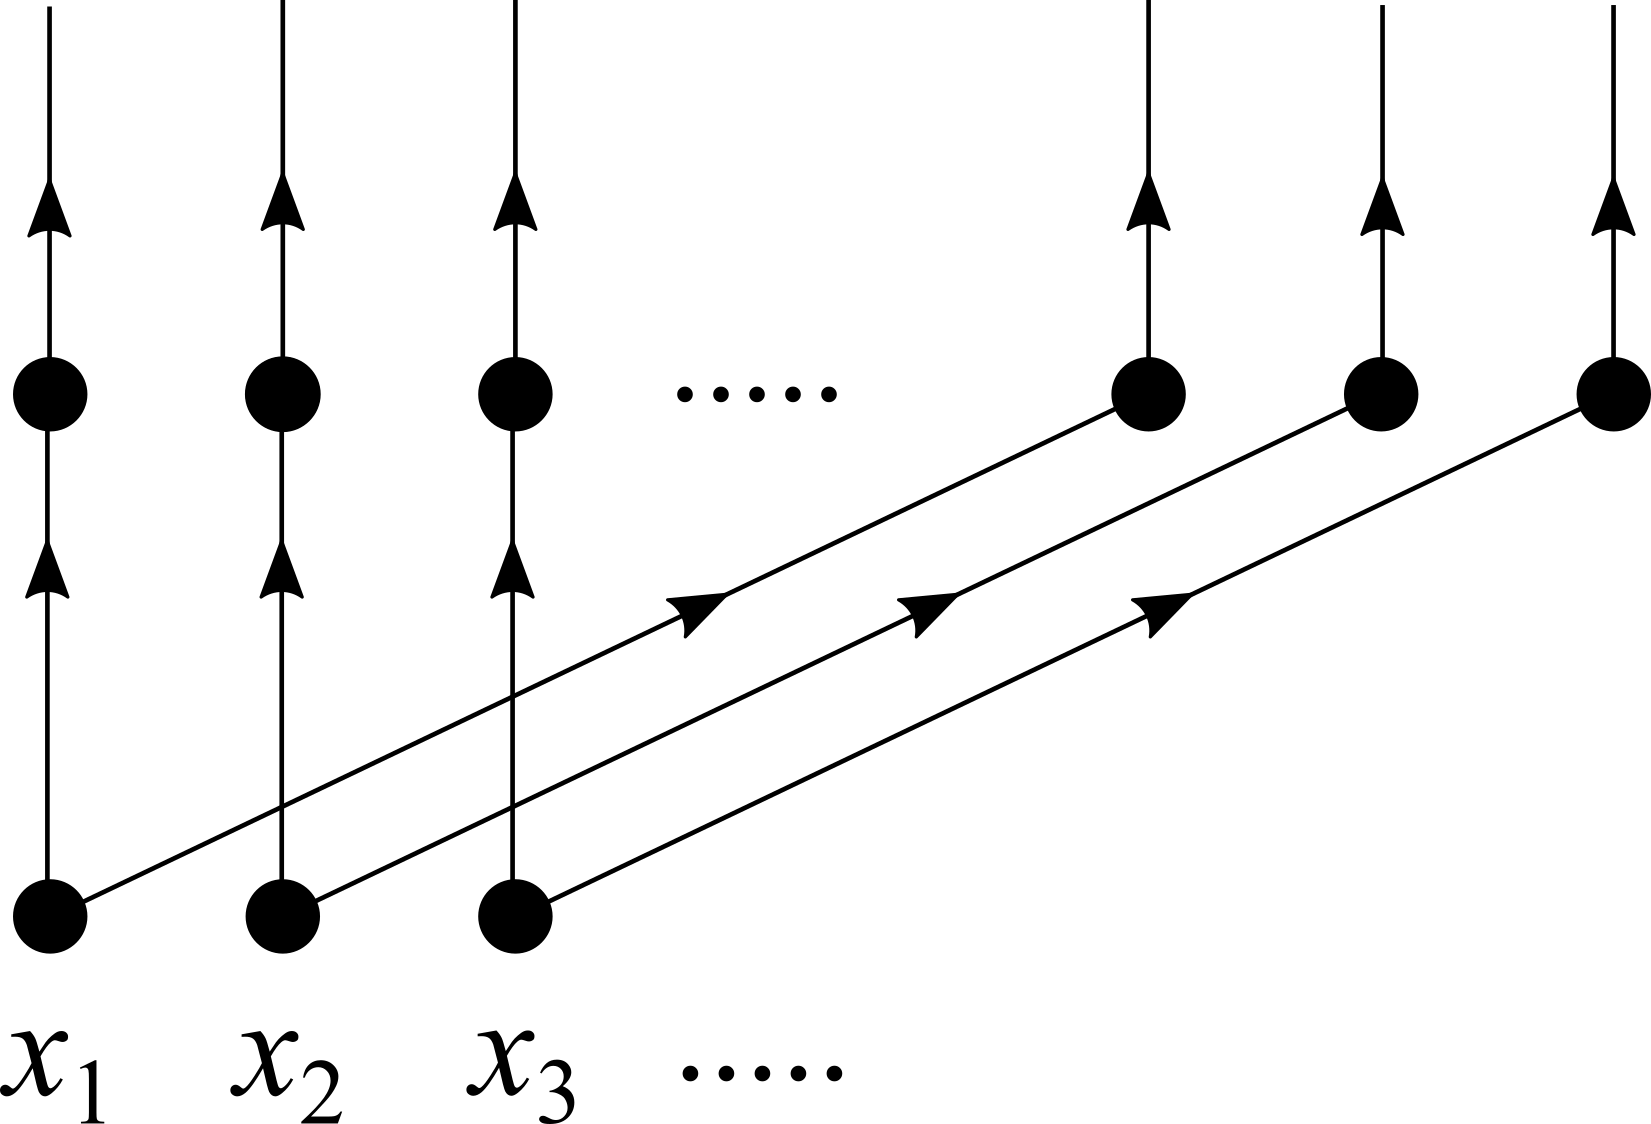
\includegraphics[scale=0.7]{NN-copying.png}}}
\end{equation}
一个输入 dim = $n$,输出 dim = $2 n$ 的神经网络,fully connected 的话需要训练 $2 n^2$ 个 weights。 但我还未有时间试验一般多层神经网络学习这个动作需要训练多久。 

其次,考虑\textbf{前件}的成立,一种可行的\textbf{几何图像}是这样的 \footnote{这只是众多可能的 representations 之一,但似乎任何「几何」形式的 representations 都有类似问题。 除非我们考虑有 ``procedural'' 特点的 representations? 以下会讨论.... }:
\begin{equation}
\vcenter{\hbox{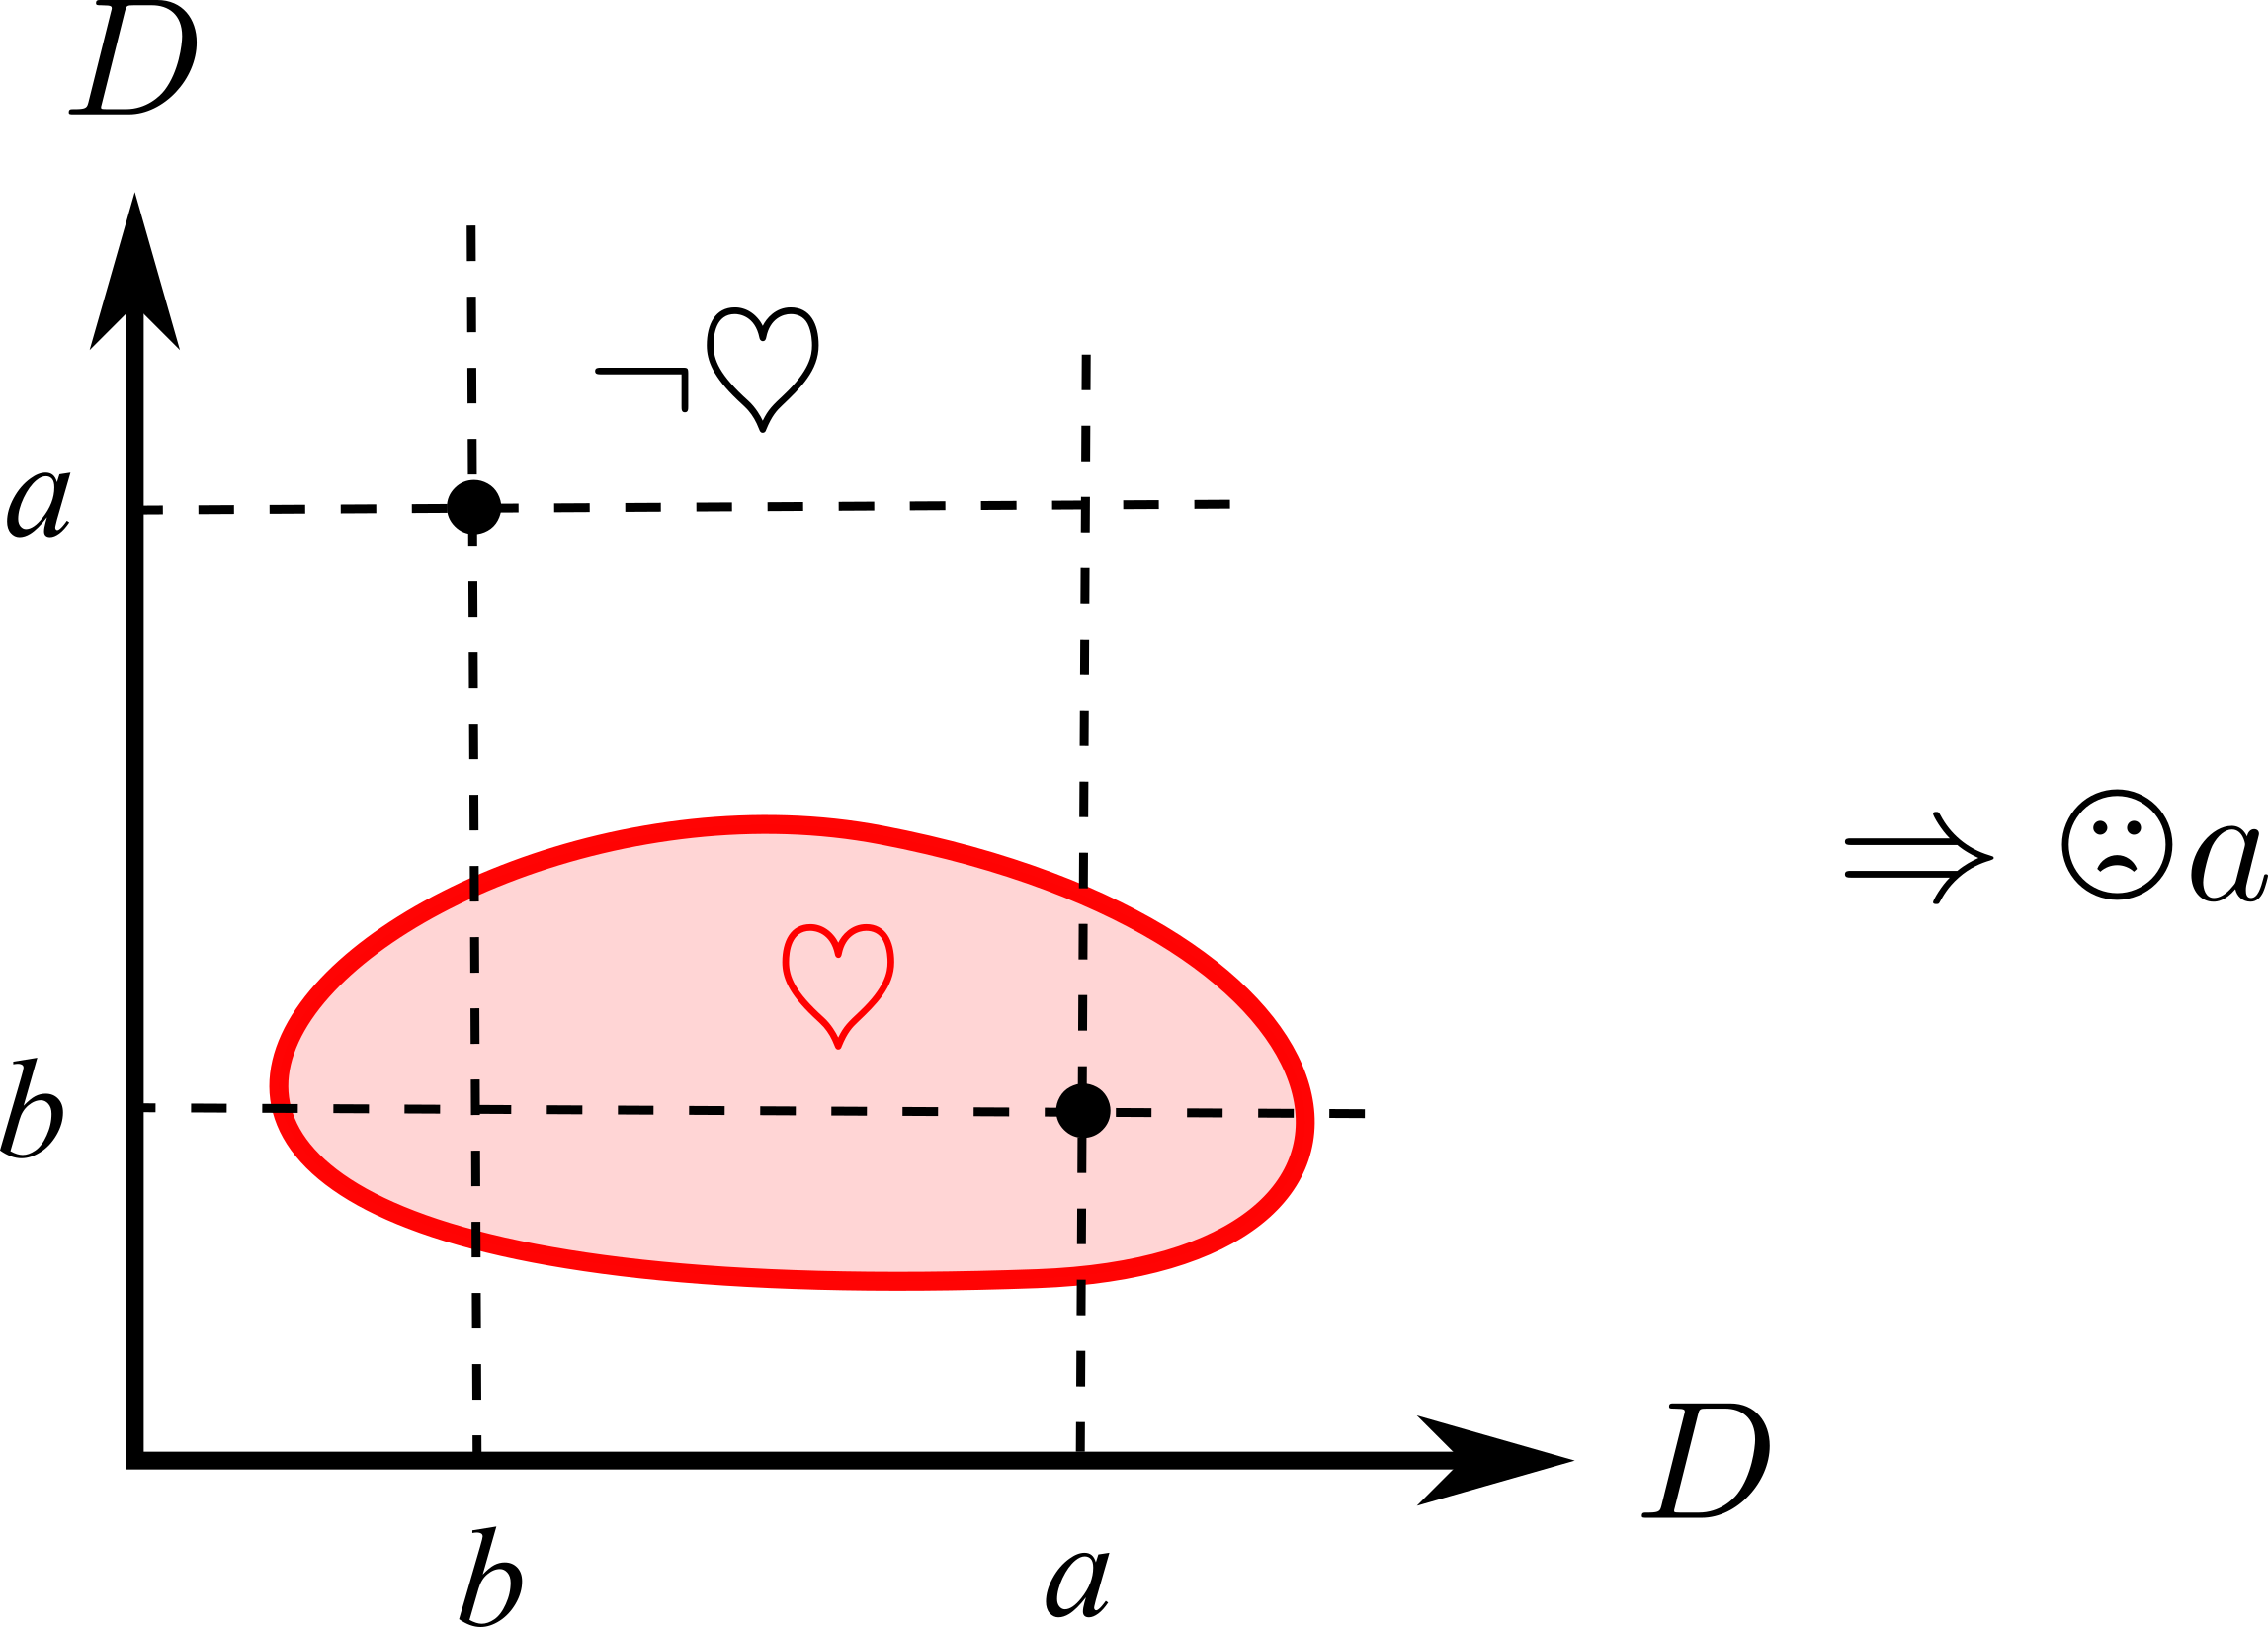
\includegraphics[scale=0.6]{heart-break.png}}}
\end{equation}
$\in$ 很容易用神经网络解决,例如可以定义 $\heartsuit$ 为一个神经网络:
\begin{equation}
\heartsuit (\vec{x}) = \begin{cases}
0 & \vec{x} \notin \mbox{region}\\
1 & \vec{x} \in \mbox{region}
\end{cases}
\end{equation}
但即使这样,仍然馀下一个 pattern matching (comparison) 问题:
\begin{eqnarray}
\vec{p}_1 = (\tikzmark{a1} \vec{a}, \vec{b} \tikzmark{b1}) &\in& \heartsuit \nonumber \\
&& \nonumber \\
\vec{p}_2 = (\tikzmark{b2} \vec{b}, \vec{a} \tikzmark{a2}) &\in& \neg \heartsuit
\begin{tikzpicture}[overlay,remember picture]
  \draw[-, red, shorten <=20pt, transform canvas={shift={(-3pt,13pt)}}] (a1.center) to (a2.center);
  \draw[-, red, shorten <=20pt, transform canvas={shift={(-6pt,13pt)}}] (a1.center) to (a2.center);
  \draw[-, red, shorten <=20pt, transform canvas={shift={(5pt,13pt)}}] (b1.center) to (b2.center);
  \draw[-, red, shorten <=20pt, transform canvas={shift={(2pt,13pt)}}] (b1.center) to (b2.center);
\end{tikzpicture}
\end{eqnarray}
以下是一个简单的用 RNN 神经网络 模拟的 comparator(所有 = 0 的权重 没有显示):
\begin{equation}
\vcenter{\hbox{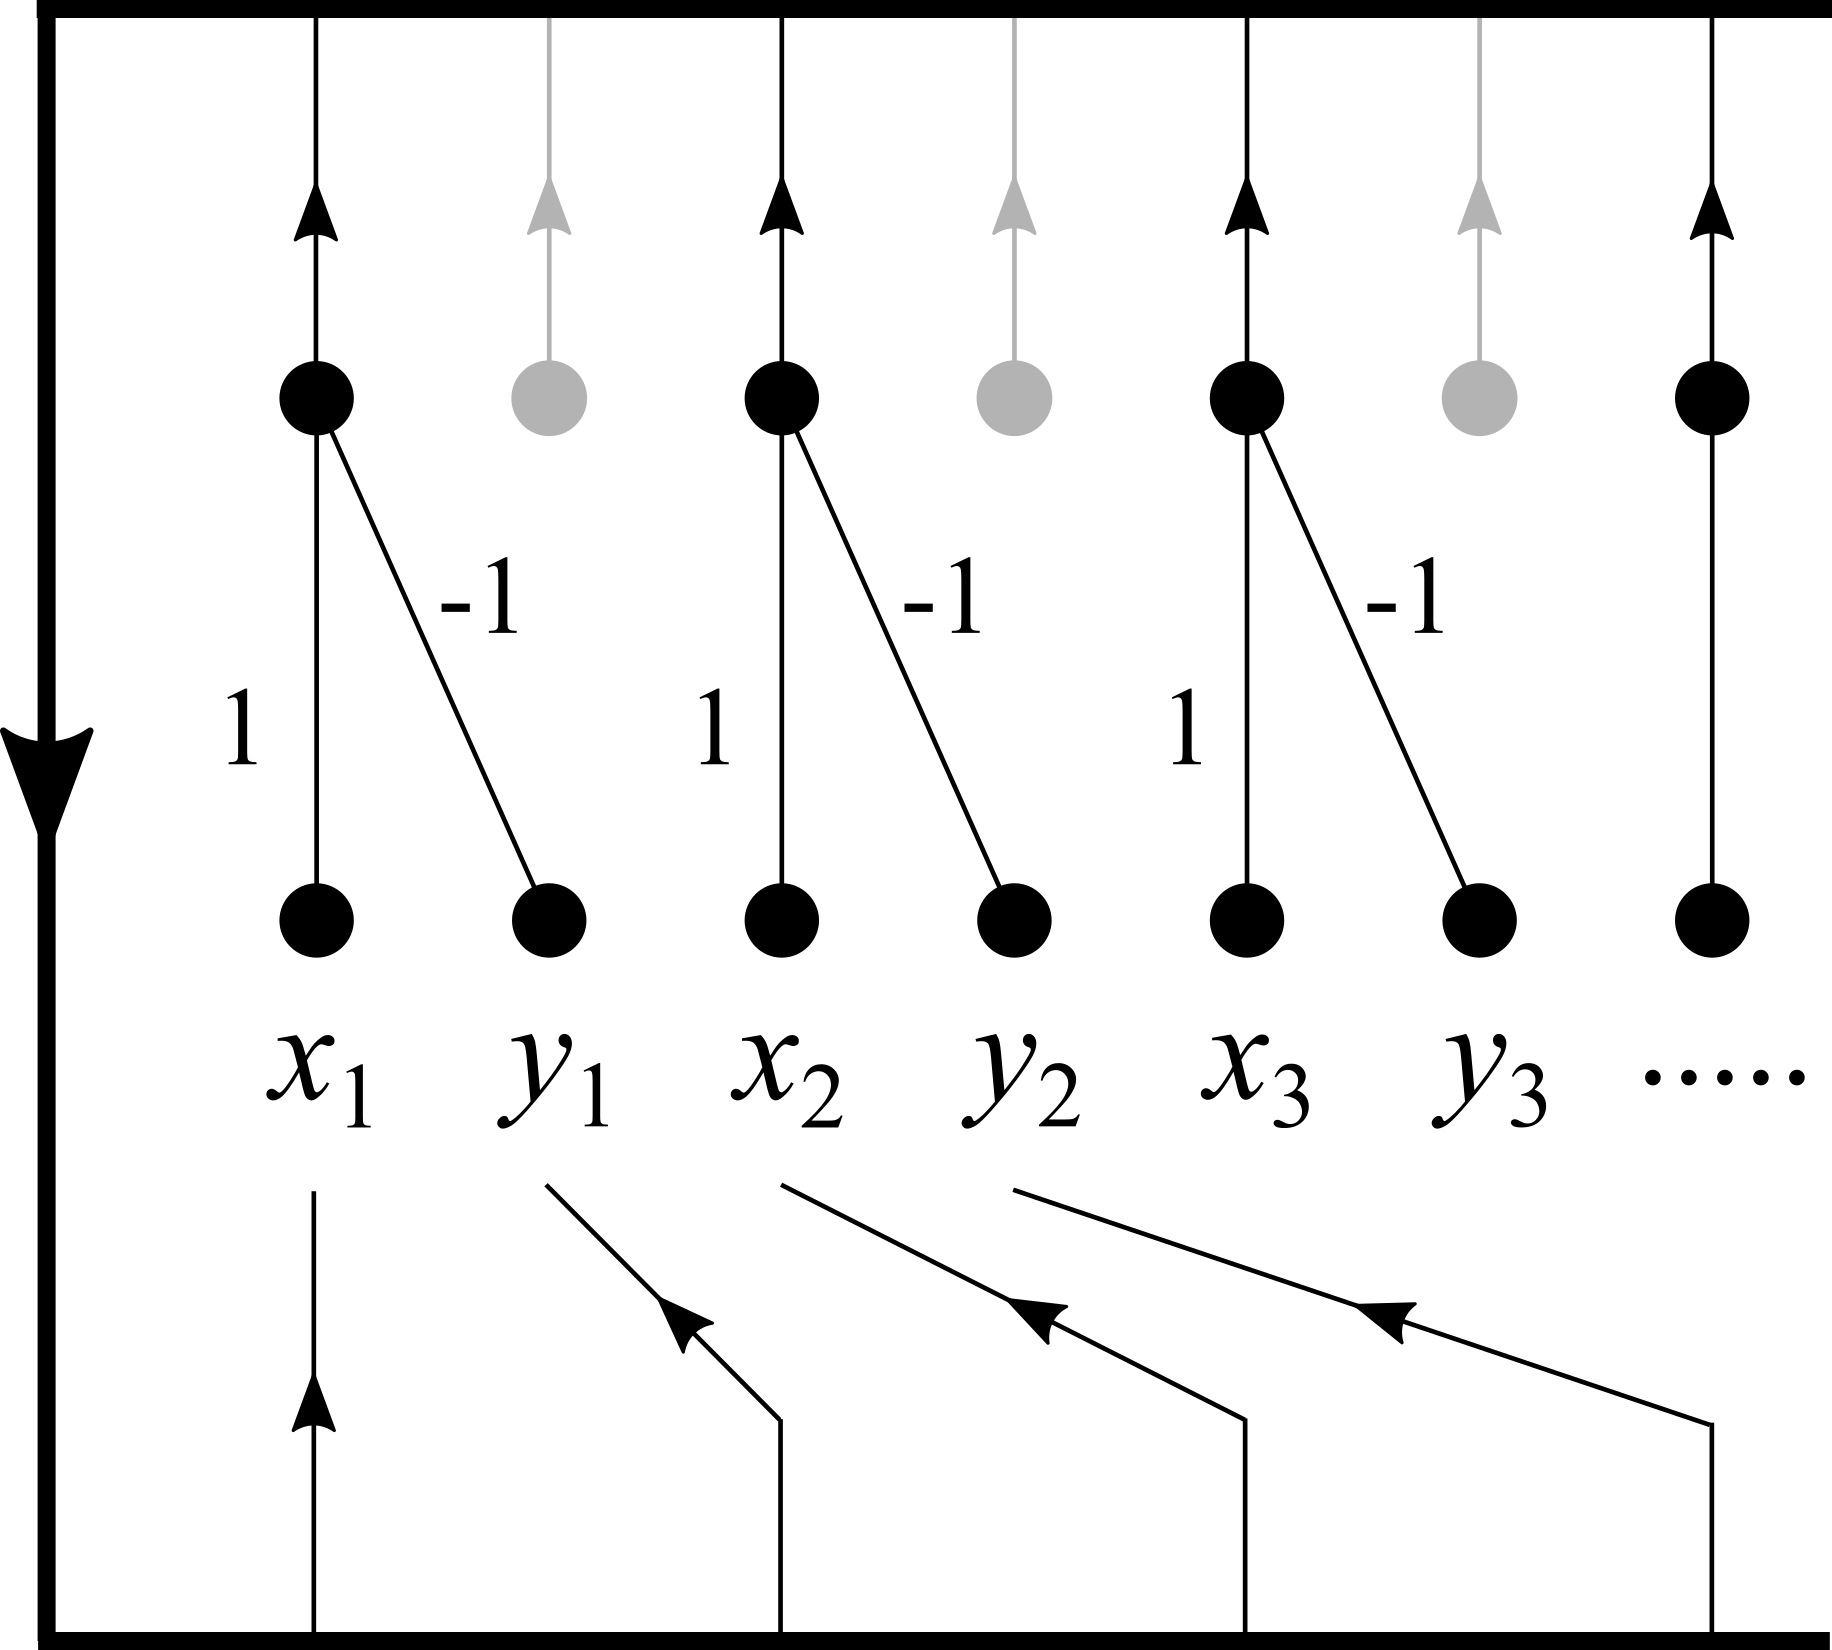
\includegraphics[scale=0.7]{NN-comparator.png}}}
\end{equation}
在 iterate $n$ 次之后,最左边的输出 会是 $\vec{x} \stackrel{?}{=} \vec{y}$ 的真假值。 假设 输入维数是 $2 n$,需要训练 $(2 n)^2$ 个 weights。

结论: 根据以上分析,用 NN 模拟 copier 和 comparator 似乎不算很难,但实际上还要将这些「元件」配合 short-term memory 使用,整个 architecture 仍然是未知的。

\subsection{「分布式」知识表述}

% Distributive representation 是针对神经网络而言的,因为神经网络是现时最强的机器学习方法(除了我最近开始提倡使用的 \textbf{基因算法})。

\textbf{Distributive representation} 的意思是: 假设有一个 vector 表示神经网络的输出端有 $n = 10$ 粒神经元:
\begin{equation}
\vec{x} = (x_1, x_2, .... , x_{10})
\end{equation}
用 2 进制,每个 $x_i \in \{ 0, 1 \}$,则 $\vec{x}$ 可以分别表示 10 个 ``\textbf{one-hot}'' 的概念。  但如果用 distributive representation,这 10 个 bits 最多可以表达 $2^n = 1024$ 个不同的状态/概念。  但其实 one-hot features 的 conjunctions 如果看成是不同的状态,则和 distributive representation 没有区别。  所以,神经网络的 representation 本质上可以说是 $\mathbb{R}^n$ vector 而已,或者看成是 $n$-维流形的 $n$ 个座标。

举例来说,\textit{``John throws ball to Mary''} 这个图像经过譬如 CNN 的处理后,可以得到一个 \textbf{分布式知识表述}:
\begin{equation}
\vcenter{\hbox{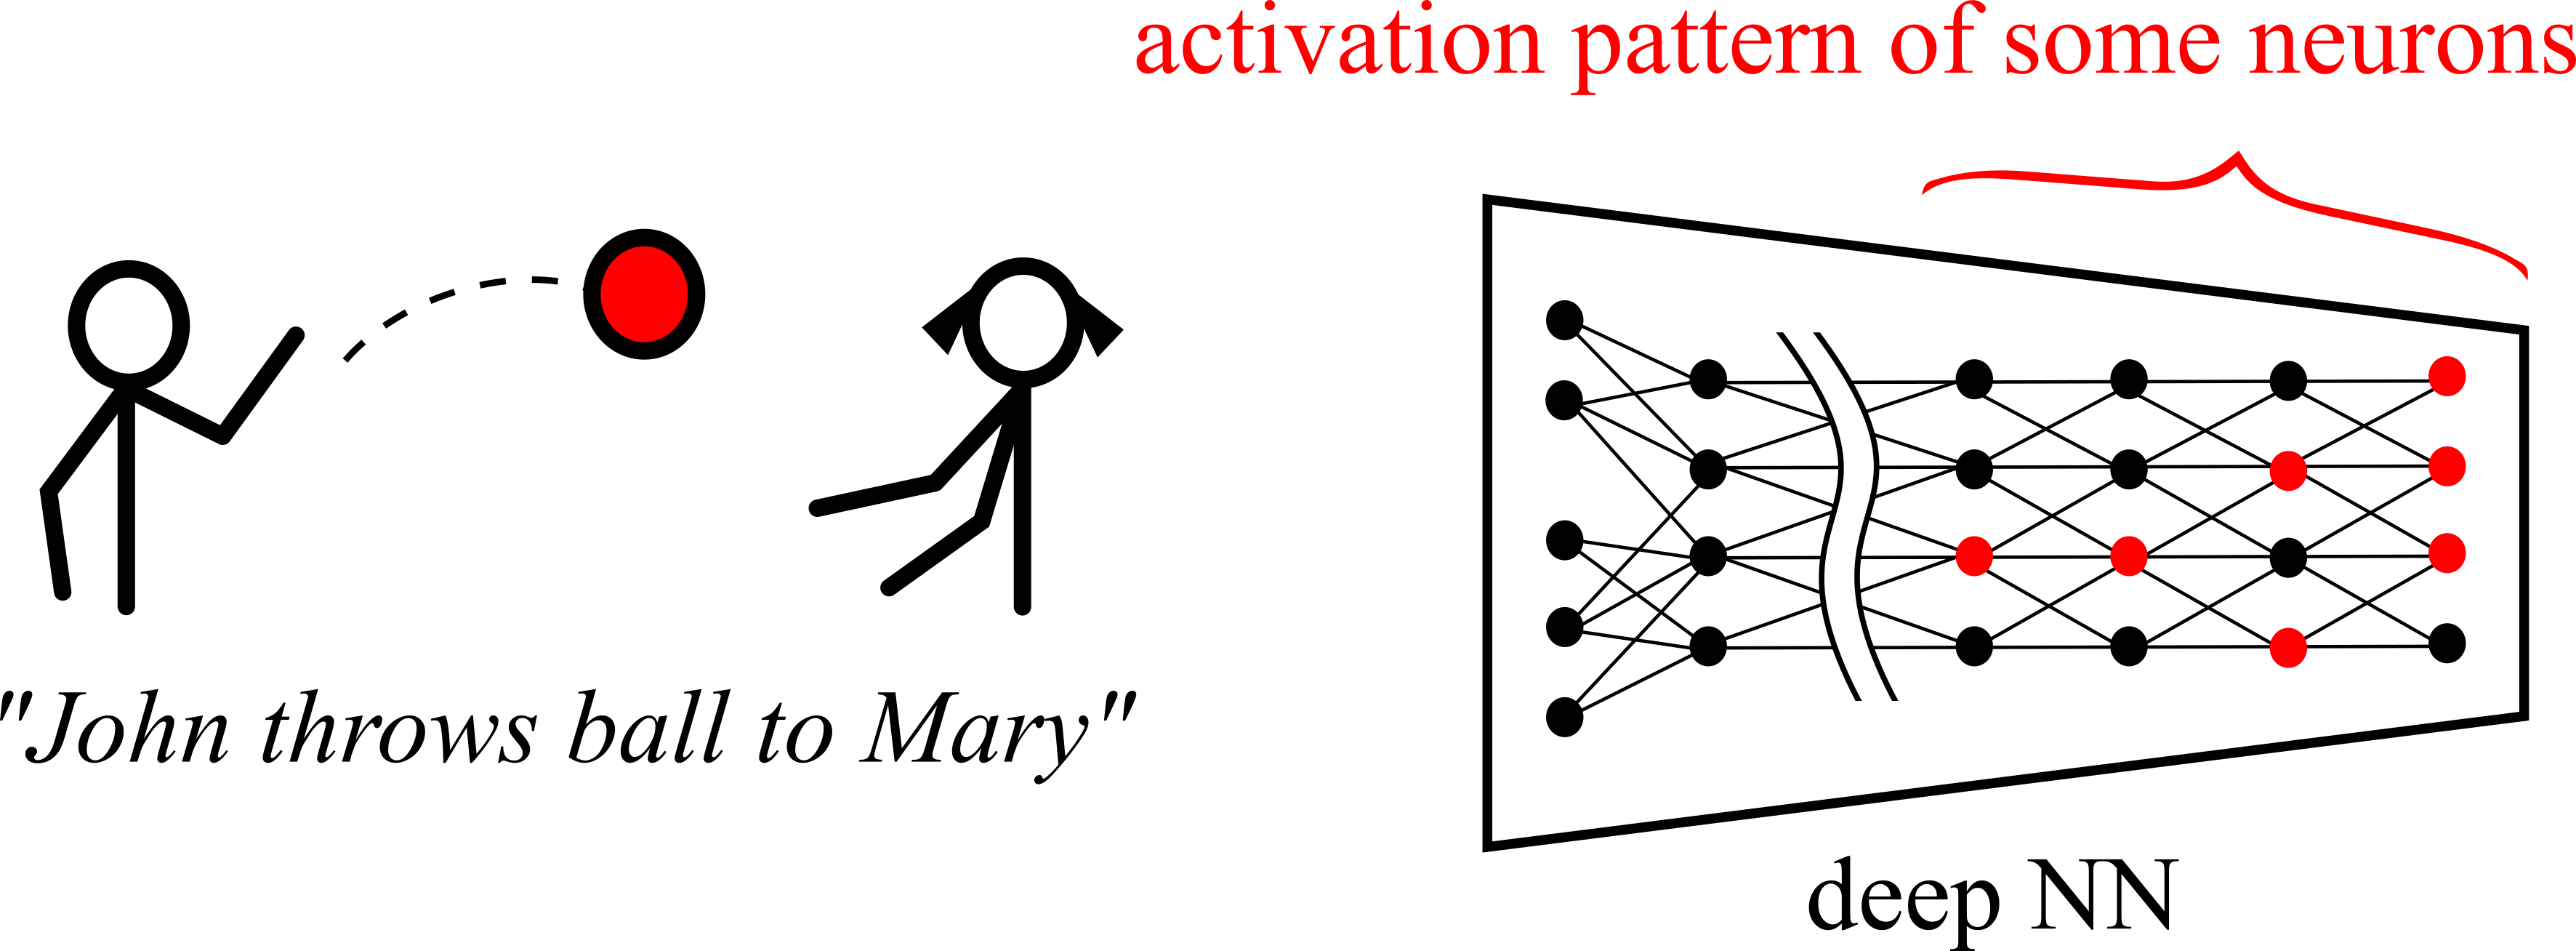
\includegraphics[scale=0.7]{NN-activation-patterns.png}}}
\end{equation}
%注意那些红点不一定是\textbf{最后}那层的输出。  这是我心目中的图像,比较 general,不是指某个特定的 implementation。  重点是: 「美女过马路」是一个 ``\textbf{neat}'' 命题,但在感知过程中,我们会认得很多细节,例如「裙子、高跟鞋、金发、斑马线、路灯」等。  这些特徵 (features) 构成整个 representation,至少我是这样理解 分布式表述 的。
这可以理解为: \uline{一个 ``neat'' 命题被分解为很多个细小的命题},例如:
\begin{equation}
\mbox{A 掷球给 B} \Longleftrightarrow \left\{
                \begin{array}{l}
                  \mbox{A手臂挥动 } \; \wedge \\
                  \mbox{球离开A的手 } \; \wedge \\
                  \mbox{球在半空飞 } \; \wedge \\
                  ...
                \end{array}
              \right.
\end{equation}
这两边是\textbf{逻辑等价}的。 在右边不能出现「球是红色的」这一细节,因为这细节不是左边\textbf{蕴涵}的。 但可以有「球通常是圆的」。 换句话说:
\begin{equation}
\boxed{\mbox{``neat'' proposition}} \quad p \Longleftrightarrow \left\{
                \begin{array}{l}
                  q_1 \; \wedge \\
                  q_2 \; \wedge \\
                  ... \; \wedge \\
                  q_n
                \end{array}
              \right.
\quad \boxed{\mbox{distributed propositions}}
\end{equation}

\textit{结论}: 未知 分布式知识表述 会给 AI 带来什么影响,暂时我们的 architectures 对 distributive 和 neat logic 同样适用,除了命题数目的增加,与及 和「视觉神经」接合 的部分。 

%经典逻辑表述是由 命题 构成的,其实 features 也可以看成是命题,例如「高跟鞋」可以看成是「有一只高跟鞋在这位置」的命题。 逻辑上来说:
%\begin{equation}
%\boxed{\mbox{neat proposition}} \quad p \Leftrightarrow \bigwedge q_i \quad \boxed{\mbox{distributive features}}
%\end{equation}
%有时(例如纯文字输入时),知道的只是一个 neat 命题,例如「美女过马路」,并不知道其他细节(例如「金发」),这时仍然可以有分布式表述,但那些特徵会是比较抽象的。

\subsection{神经网络 缺乏短期记忆}

考虑「白猫追黑猫」这个图像:
\begin{equation}
\vcenter{\hbox{
\includegraphics[scale=0.7]{white-cat-chase-black-cat.png}}}
\end{equation}
「猫」的概念需要出现 \textbf{两次},但神经网络内对应於「猫」的特徵只有 \textbf{一组}(除非有两个重复的可以表示任何概念的 modules,但很浪费)。 换句话说,现时的 CNN 没有「巡迴 (traverse)」视野域的能力; \uline{它不能辨别和描述物体之间的 }\textbf{\uline{关系}}。 

很难想像一个 ``monolithic'' neural module (例如 feed-forward NN 或 RNN)怎样可以做到这功能。 似乎必须将命题表述成一连串 概念 的 \textbf{时间序列} (time sequence),即某种 \textbf{短期记忆} (\textbf{STM}, short-term memory)。

我有点惊讶地发现,目前 神经网络 没有 \textbf{短期记忆} 的机制,「短期」意思是在 time-scale 上短於 weights 改变的时间。 例如我告诉你一串数字(例如电话号码),你可以在脑中记住它,但这个机制在现时人工神经网络里面似乎没有研究,或许在 computational neuroscience 里面有些模型,但暂时我不清楚。  缺乏这种 STM,则很难模拟 symbolic logic,换句话说,做不到强人工智能。 

例如用 NN 实现一个 \textbf{动态的记忆体},它接收新来的元素时,会对记忆体中其他元素逐一 \textbf{比较},而且具备 \textbf{复制} 功能。  例如以下这个像「迴转木马」的时间序列机制(每个 $\NewSym{distributive-vector.png}$ 代表一支 distributive vector):
\begin{equation}
\vcenter{\hbox{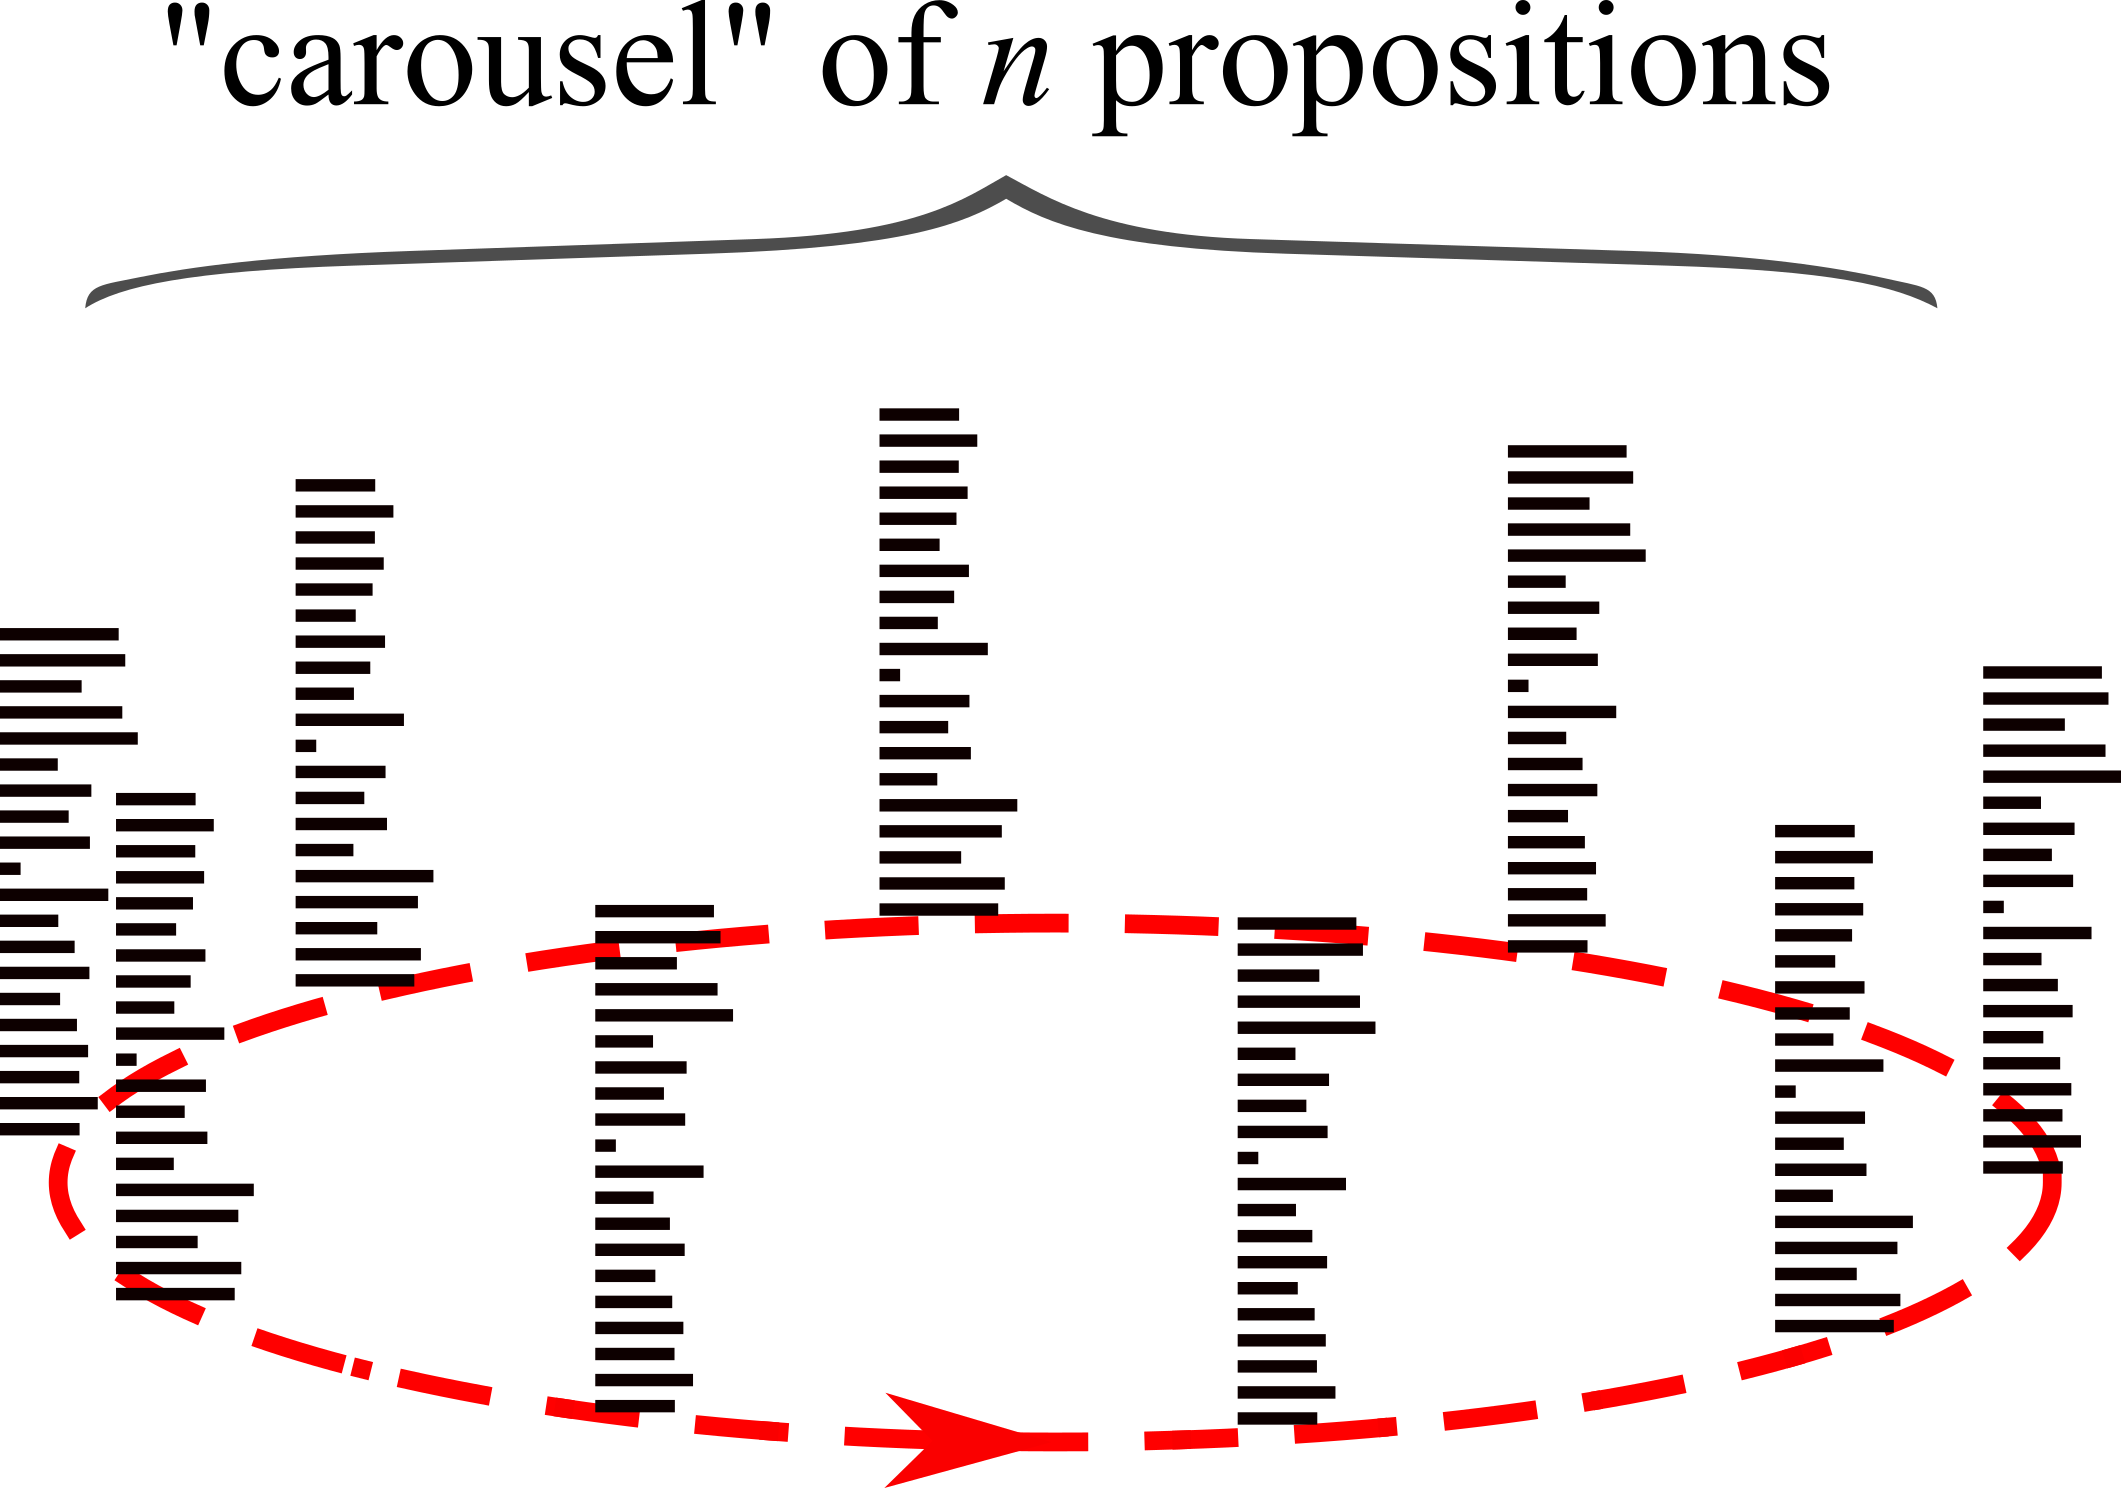
\includegraphics[scale=0.7]{carousel-of-vectors.png}}}
\end{equation}
总之,纯粹用 NN 模拟 STM,明显地很麻烦。

%\begin{tcolorbox}[breakable, colback=yellow]
%用神经网络解决强人工智能的最大障碍是 从命题逻辑到一阶逻辑的\textbf{跃升},特别是 substitution 运算,需要有 short-term memory 机制
% The bottleneck of strong AI is the \textbf{learning algorithm}'s speed, and the most crucial obstruction is the \textbf{lifting} from propositional to first-order logic.
%\end{tcolorbox}

\subsection{Graph neural networks}
\label{graph-NN}

\begin{tcolorbox}[ams equation, colback=yellow, colframe=white]
\mbox{用 graph 做记忆体(包括短期和长期记忆)}
\end{tcolorbox}
而在增加新记忆单元时,相同的 nodes 会被 match 成一个,换句话说 matching 这步骤用传统 symbolic 方法解决,馀下的问题再交给 神经网络。 
\begin{eqnarray}
\mbox{model } \mathcal{M} &=& \mbox{graph} \nonumber \\
\mbox{rewriter} &=& \mbox{deep NN = graph neural network}
\end{eqnarray}

很多谢 Google / DeepMind 在 2018 年 6 月发表的 graph network 论文 \parencite{Battaglia2018},Peter Battaglia 和 26 名合作者 survey 了 graph network 的发展情况。  他们提出的 graph network 更接近一些 physical system 例如 弹簧和球体 的系统,而不是 first-order 的模型,但本质上是一样的。

通常 model 太大,需要用 attention mechanism 选取它的一个 fragment,再 ``present'' 给 神经网络 处理:
\begin{equation}
\vcenter{\hbox{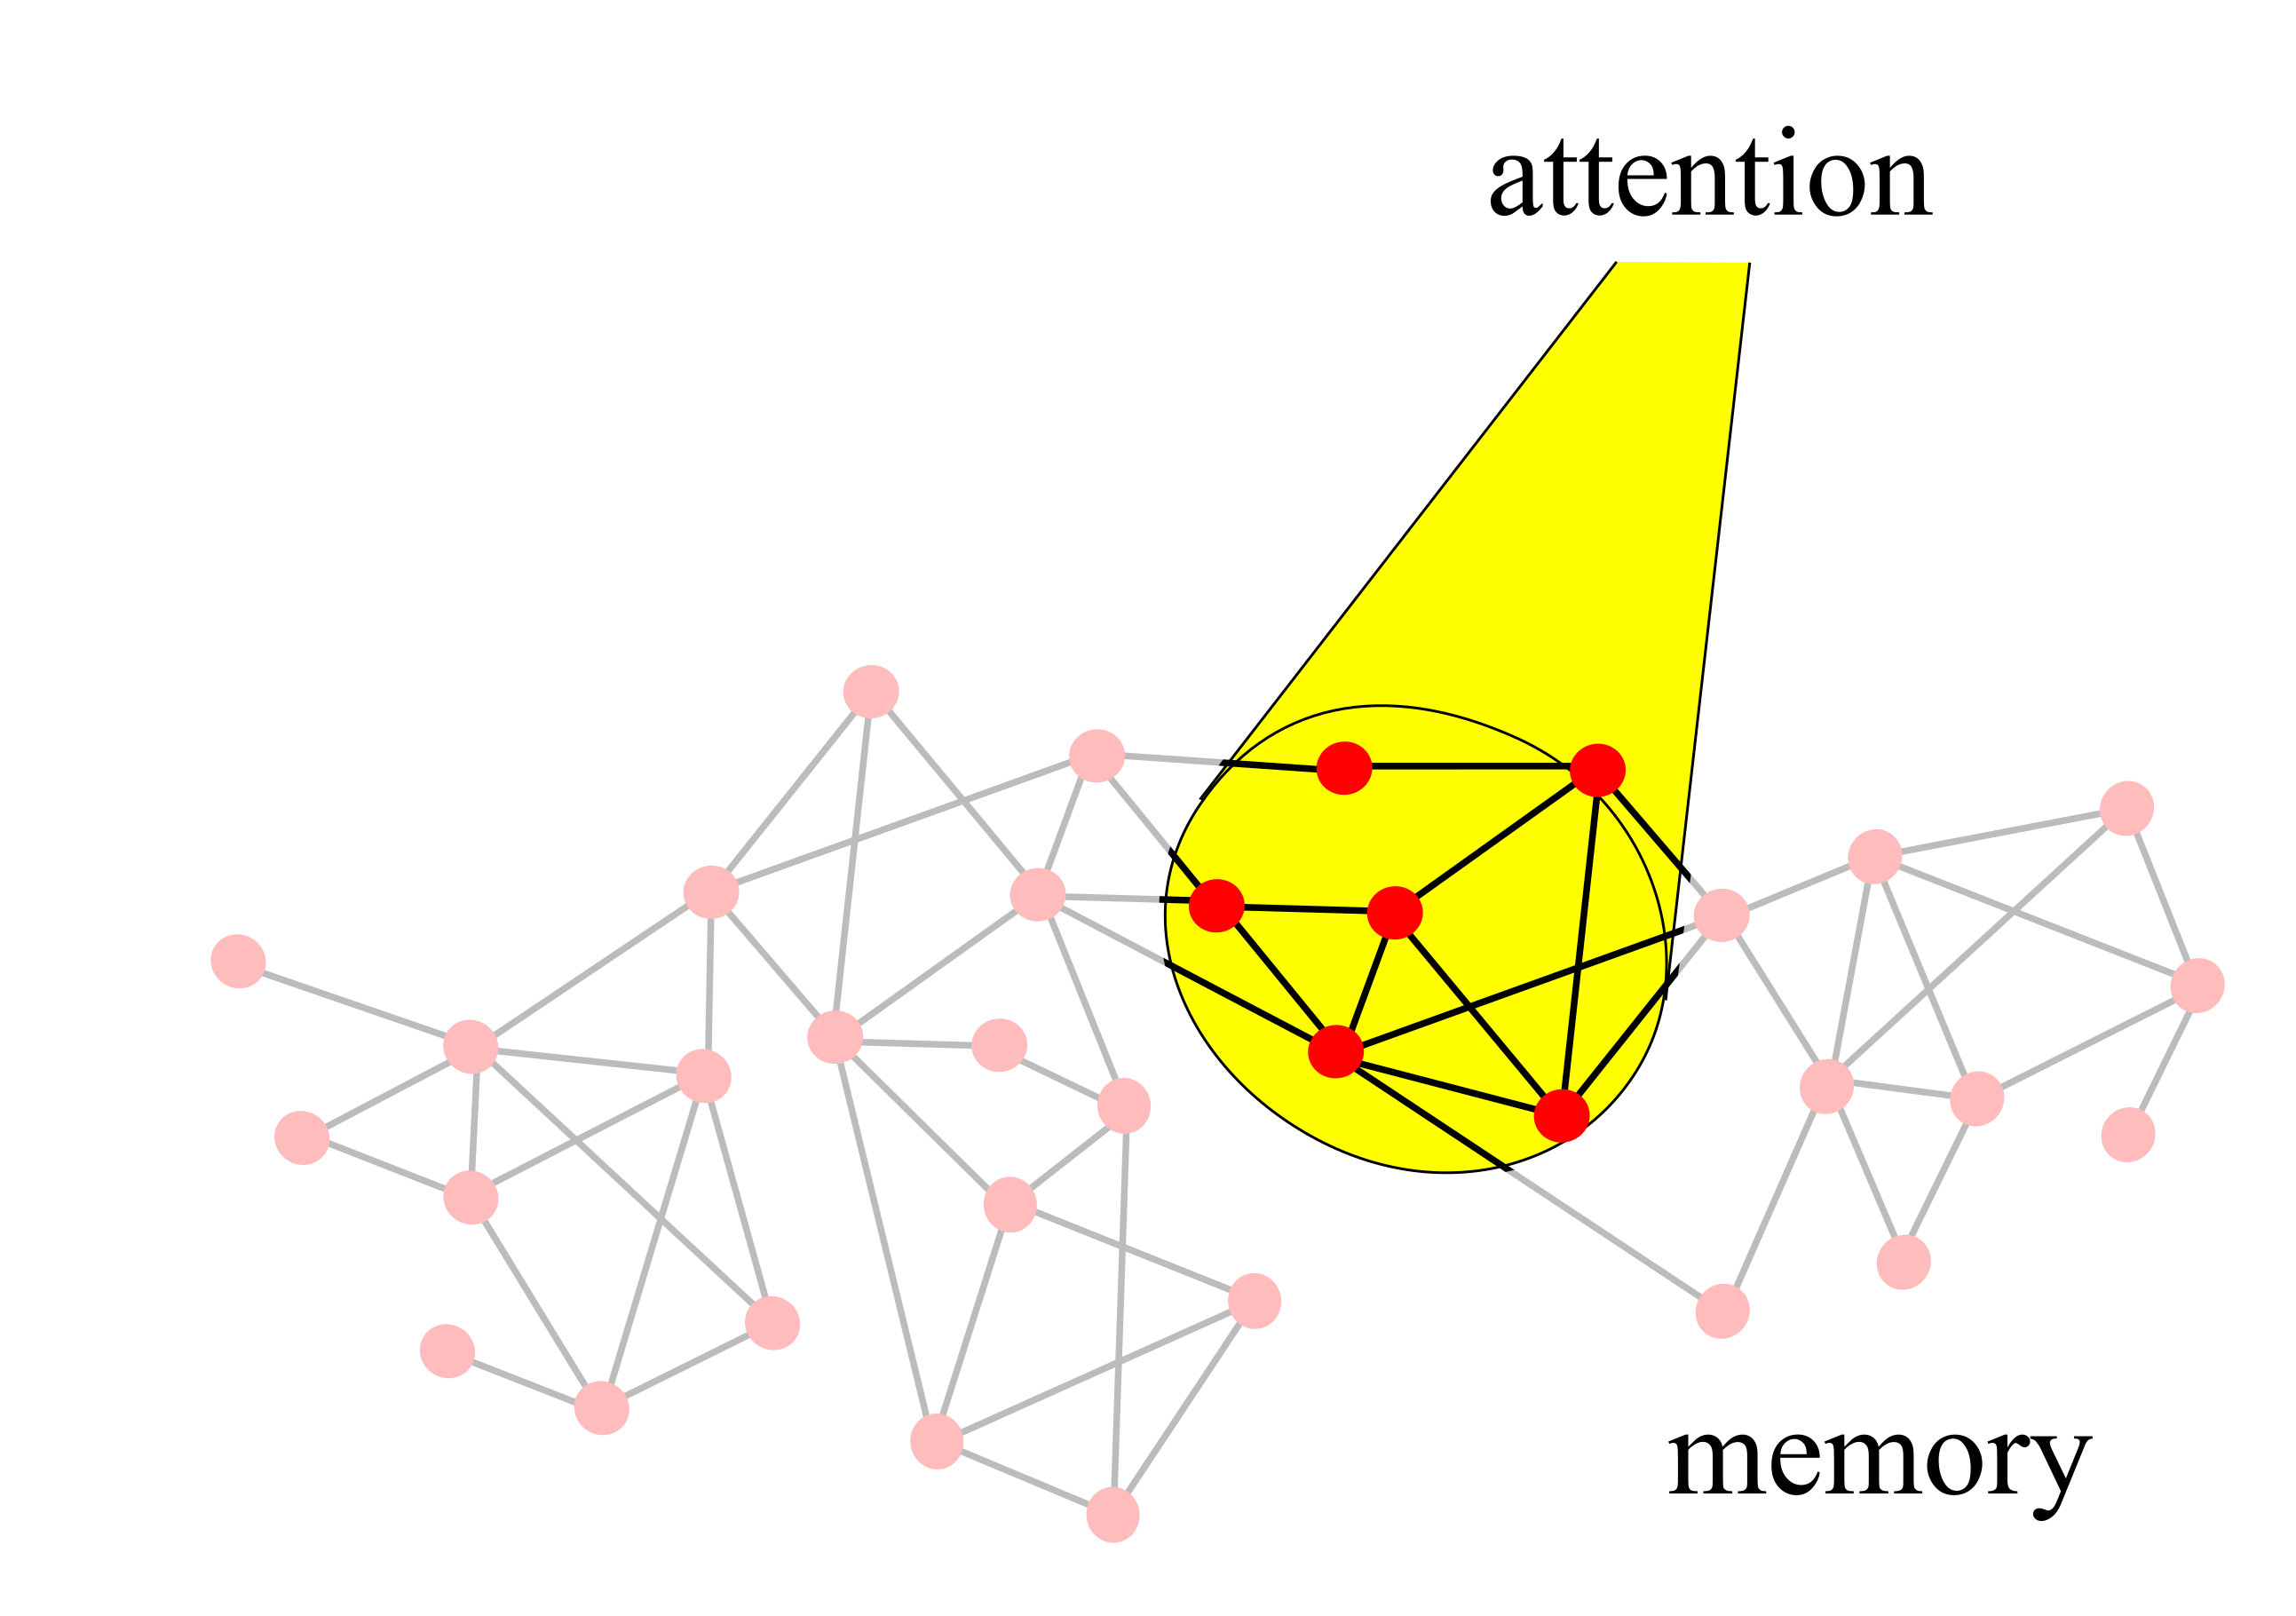
\includegraphics[scale=0.7]{attentional-mechanism.png}}}
\end{equation}
这 attention mechanism 和 现时 深度学习 里面的 attention 或者在具体细节上有些分别,但基本上是同一概念。 

神经网络的输入 $\vec{x}$,需要这样的一个 embedding:
\begin{equation}
\boxed{\mbox{graph}} \quad
\begin{tikzcd}[column sep = large]
\NewSym[1.5]{../graph-symbol.png} \ar[r, hookrightarrow, "\mbox{embed}"] & (x_1, ..., x_n) 
\end{tikzcd}
\quad \boxed{\mbox{vector}}
\end{equation}
但 graph 并不是一个「线性」的结构 \footnote{线性是指符号形式上,例如 tree 可以表示成线性的一行},将 graph 结构表示成一支 vector 似乎颇难(这或许是 graph neural networks 迟迟未有突破的原因)。  

\begin{tcolorbox}[breakable, parbox=false]
数学表示论里面有 \textbf{quiver representations},它将 vertex 变成 vector space,edge 变成 linear transformation between vector spaces. 例如:
\begin{equation}
\begin{tikzcd}[column sep = large]
\mbox{John} \arrow[r, bend left, "\heartsuit"] & \arrow[l, bend left, swap, "\neg \heartsuit"] \mbox{Mary}
\end{tikzcd}
\quad \Longrightarrow \quad
\begin{tikzcd}[column sep = large]
V_1 \arrow[r, bend left, "M_1"] & \arrow[l, bend left, "M_2"] V_2
\end{tikzcd}
\end{equation}
其中 $V_1, V_2$ 是向量空间,$M_1, M_2 \in GL(\mathbb{R})$ 是 矩阵。  但这仍然不是一支向量。  

在 向量空间 $V_i$ 的 \textbf{基底变换}下,两个矩阵 $M$ 可能是同一个线性变换。  故需要考虑它们的\textbf{不变性},亦即 moduli。 表示论 关心的是 将各种 $M$ \uline{分解成不可约成分}。 这分解里出现的 Dynkin diagrams 和 Lie algebra 分类时出现的一样。  但如果 quiver 不是 Dynkin 或某些扩充,则这 quiver 是 ``wild'' 的,很难分解。 即使很简单的 quiver 也可以是 wild type。

每个 quiver 定义一个 path algebra,它的元素是 quiver 里的 path,换句话说即是逻辑上的 \textbf{关系} 及其 compositions。 暂时不知道 quiver representations 在 AI 里有什么用。
\end{tcolorbox}

解决办法: 现时 在 自然语言理解 方面 最强的深度学习模型,据我所知是基於 CNN 或 RNN 的模型,而它们处理的是线性的 sequence 输入。 所以要将 memory graph 分拆成线性的元素(亦即个别的 关系/命题),而且里面不可以用 global variable references(换句话说,已经进行了 variable matching 处理)。  然后 NN 输出的 variable copying 也是 externally 处理的。 换句话说,用 ``hybrid'' 的方式,结合 NN 和 \textbf{graph rewriting}。

注意: 虽然 NN 的参数空间 $\Theta$ 是 \textbf{连续}的,但它 learn 出来的 rewriting rules 却是 \textbf{离散}的,因为 graph 本身是个 离散结构。 

补充一点: attention mechanism 要 traverse memory graph,换句话说是一种 graph search algorithm,这部分可以和 NN 结合成同一个 module(现时有很多 RNN architectures 就是这样)。

馀下 2 节是一些 数学 背景知识....
\hrule

\section{Categorical semantics}
\label{Categorical-semantics}

Categorical semantics 是用 category theory 表达的 model theory。  以下内容主要来自 \parencite{Caramello2018} 这本新书的第一章。  更经典的参考书是 \parencite{Goldblatt2006}. 

不同的 logics 可以透过 \textbf{proof theory}(它研究的是 \textit{syntactic} rules of deduction)定义:
\begin{equation}
\begin{tabular}{|l|l|}
\hline
algebraic logic & no additional rules\\
\hline
Horn logic & finite $\wedge$ \\
\hline
regular logic & finite $\wedge$, $\exists$, Frobenius axiom\\
\hline
coherent logic & finite $\wedge$ and $\vee$, $\exists$,\\
				& distributive axiom, \\
				& Frobenius axiom \\
\hline
geometric logic & finite $\wedge$, infinitary $\vee$, $\exists$,\\
				& infinitary distribution axiom,\\
				& Frobenius axiom \\
\hline
first-order intuitionistic logic & all finitary rules \\
				& except law of excluded middle\\
\hline
first-order classical logic & all finitary rules \\
\hline
\end{tabular}
\end{equation}

举例来说,\textbf{algebraic theory} 的意思是: 它只有一个 relation $=$,而所有 axioms 都是 $s = t$ 这种形式。 

还有这些 deduction rules 的例子:
\begin{equation}
\boxed{\wedge \mbox{ rule}}	\quad \frac{\Phi \vdash \Psi, \; \Phi \vdash \Chi}{\Phi \vdash (\Psi \wedge \Chi)}
\end{equation}
\vspace*{-5pt}
\begin{equation}
\boxed{\exists \mbox{ double rule}}	\quad \Dfrac{\Phi \vdash_{\vec{x}, y} \Psi}{\exists y \, \Phi \vdash_{\vec{x}} \Psi}
\end{equation}
\begin{equation}
\boxed{\mbox{Frobenius axiom}}	\quad \Phi \wedge \exists y \, \Psi \vdash_{\vec{x}} \exists y \, (\Phi \wedge \Psi)
\end{equation}

Tarski 的模型论 将 first-order syntax 「对应」到 集合论 的 \textbf{结构} (structures) 上。  由此推广,不同的 逻辑 syntax 对应於不同的 结构范畴:
\begin{equation}
\begin{tabular}{|l|l|}
\hline
categories with finite products & algebraic logic \\
\hline
Cartesian categories			& Cartesian logic \\
\hline
regular categories				& regular logic \\
\hline
coherent categories				& coherent logic \\
\hline
geometric categories			& geometric logic \\
\hline
Heyting categories				& first-order intuitionistic logic \\
\hline
Boolean coherent categories		& first-order classical logic \\
\hline
\end{tabular}
\end{equation}

``Geometric'' logic 的意思来自 \textbf{geometric morphisms},它可以粗略地理解为两个 topoi 之间的映射,类似於 \textbf{continuous maps} between topological spaces。 

\uline{Topos 可以理解为 set theory 受范畴论影响下的一种推广}。 每个 elementary topos\footnote{Elementary 是集合中「元素」的意思} 有一个 \textbf{sub-object classifier} $\Omega$.  $\Omega$ 是一个特殊的 object,例如 $\{ \top, \bot \}$,代表 \textbf{真 假} 二值。 用 $\Omega$ 可以定义 sub-objects 亦即集合论中的 \textbf{子集} 概念。  举例来说,``Love'' 是一个在 $D \times D$ 内的 \textbf{关系},$D$ 是所有「人」的集合。  可以将 $D \times D$ 看成是 full relation,则 $\mbox{Love} \subset D \times D$ 是它的\textbf{子集}。  换句话说,这是 elementary topos 可以用来做 relation algebra 或 first-order logic 的 \textbf{模型} 的原因。 (参见 \parencite{Goldblatt2006})

一些历史: 在 1963 年左右,topos 的概念独立地来自几个不同的发源地: Alexander Grothendieck 在代数几何方面发展的 sheaf theory,和 F William Lawvere 用范畴论重新表述集合论,还有 Paul Cohen 的 forcing 理论(后者用来解决 \textbf{连续统假设})。  Sheaf 的意思是: 在一些 open sets $V_i$ 上定义的物体,它们在 overlap $V_i \cap V_j$ 上是吻合的,即可以 ``collate'',情形就像微分几何里一些 charts 拼合成 atlas。  二战后,Leray,接著 Cartan,用 open sets 的方法定义了 sheaf。 其后 Lazard 用 \'{e}tale 定义 sheaf,后者是 topos 理论的主要动机。  例如,一个范畴 $\mathcal{A}$ 上的 pre-sheaf 可以定义为一个 \textbf{functor}:
\begin{equation}
\mathcal{A}^{\mathrm{op}} \rightarrow \mathbf{Set}
\end{equation}
Grothendieck 将 sheaf 应用在 topology (cohomology)上,而后 Jean-Pierre Serre 发现它也可以用在代数几何上,他们和其他合作者 写了 1623 页的巨著 《SGA IV》,重大影响了代数几何的发展,导致 1974 年 Deligne 解决了 Weyl 猜想。  但我暂时不熟悉代数几何,所以不太清楚 Grothendieck 他们做了什么.... 详细可参看 \parencite{MacLane1992} 一书。

在拓樸空间上,一个 open set $U$ 的 complement 是 closed 而且未必 open,所以如果局限在 open sets 之内,则 $U$ 的 ``negation'' 应该定义为 ``the interior of its complement''.  这导致 $U$ 的「\textbf{双重否定}」不一定等於 $U$,换句话说,\uline{the algebra of open sets follows \textbf{intuitionistic logic}}, such an algebra is called a \textbf{Heyting algebra}.  (参考书同上)

Topoi 之间有两种 morphisms: \textbf{geometric morphisms} 和 \textbf{logical functors}.  前者保持「几何结构」,后者保持逻辑上的 type theory,所以有 \textbf{elementary topos} 的定义。 后者的特点是它有 \textbf{sub-object classifier} $\Omega$。 

以下是根据 \parencite{Caramello2018} Ch.1 整理出来的一张关系图,但我暂时还不太熟悉范畴论的概念,所以也不完全理解: 
\begin{equation}
\vcenter{\hbox{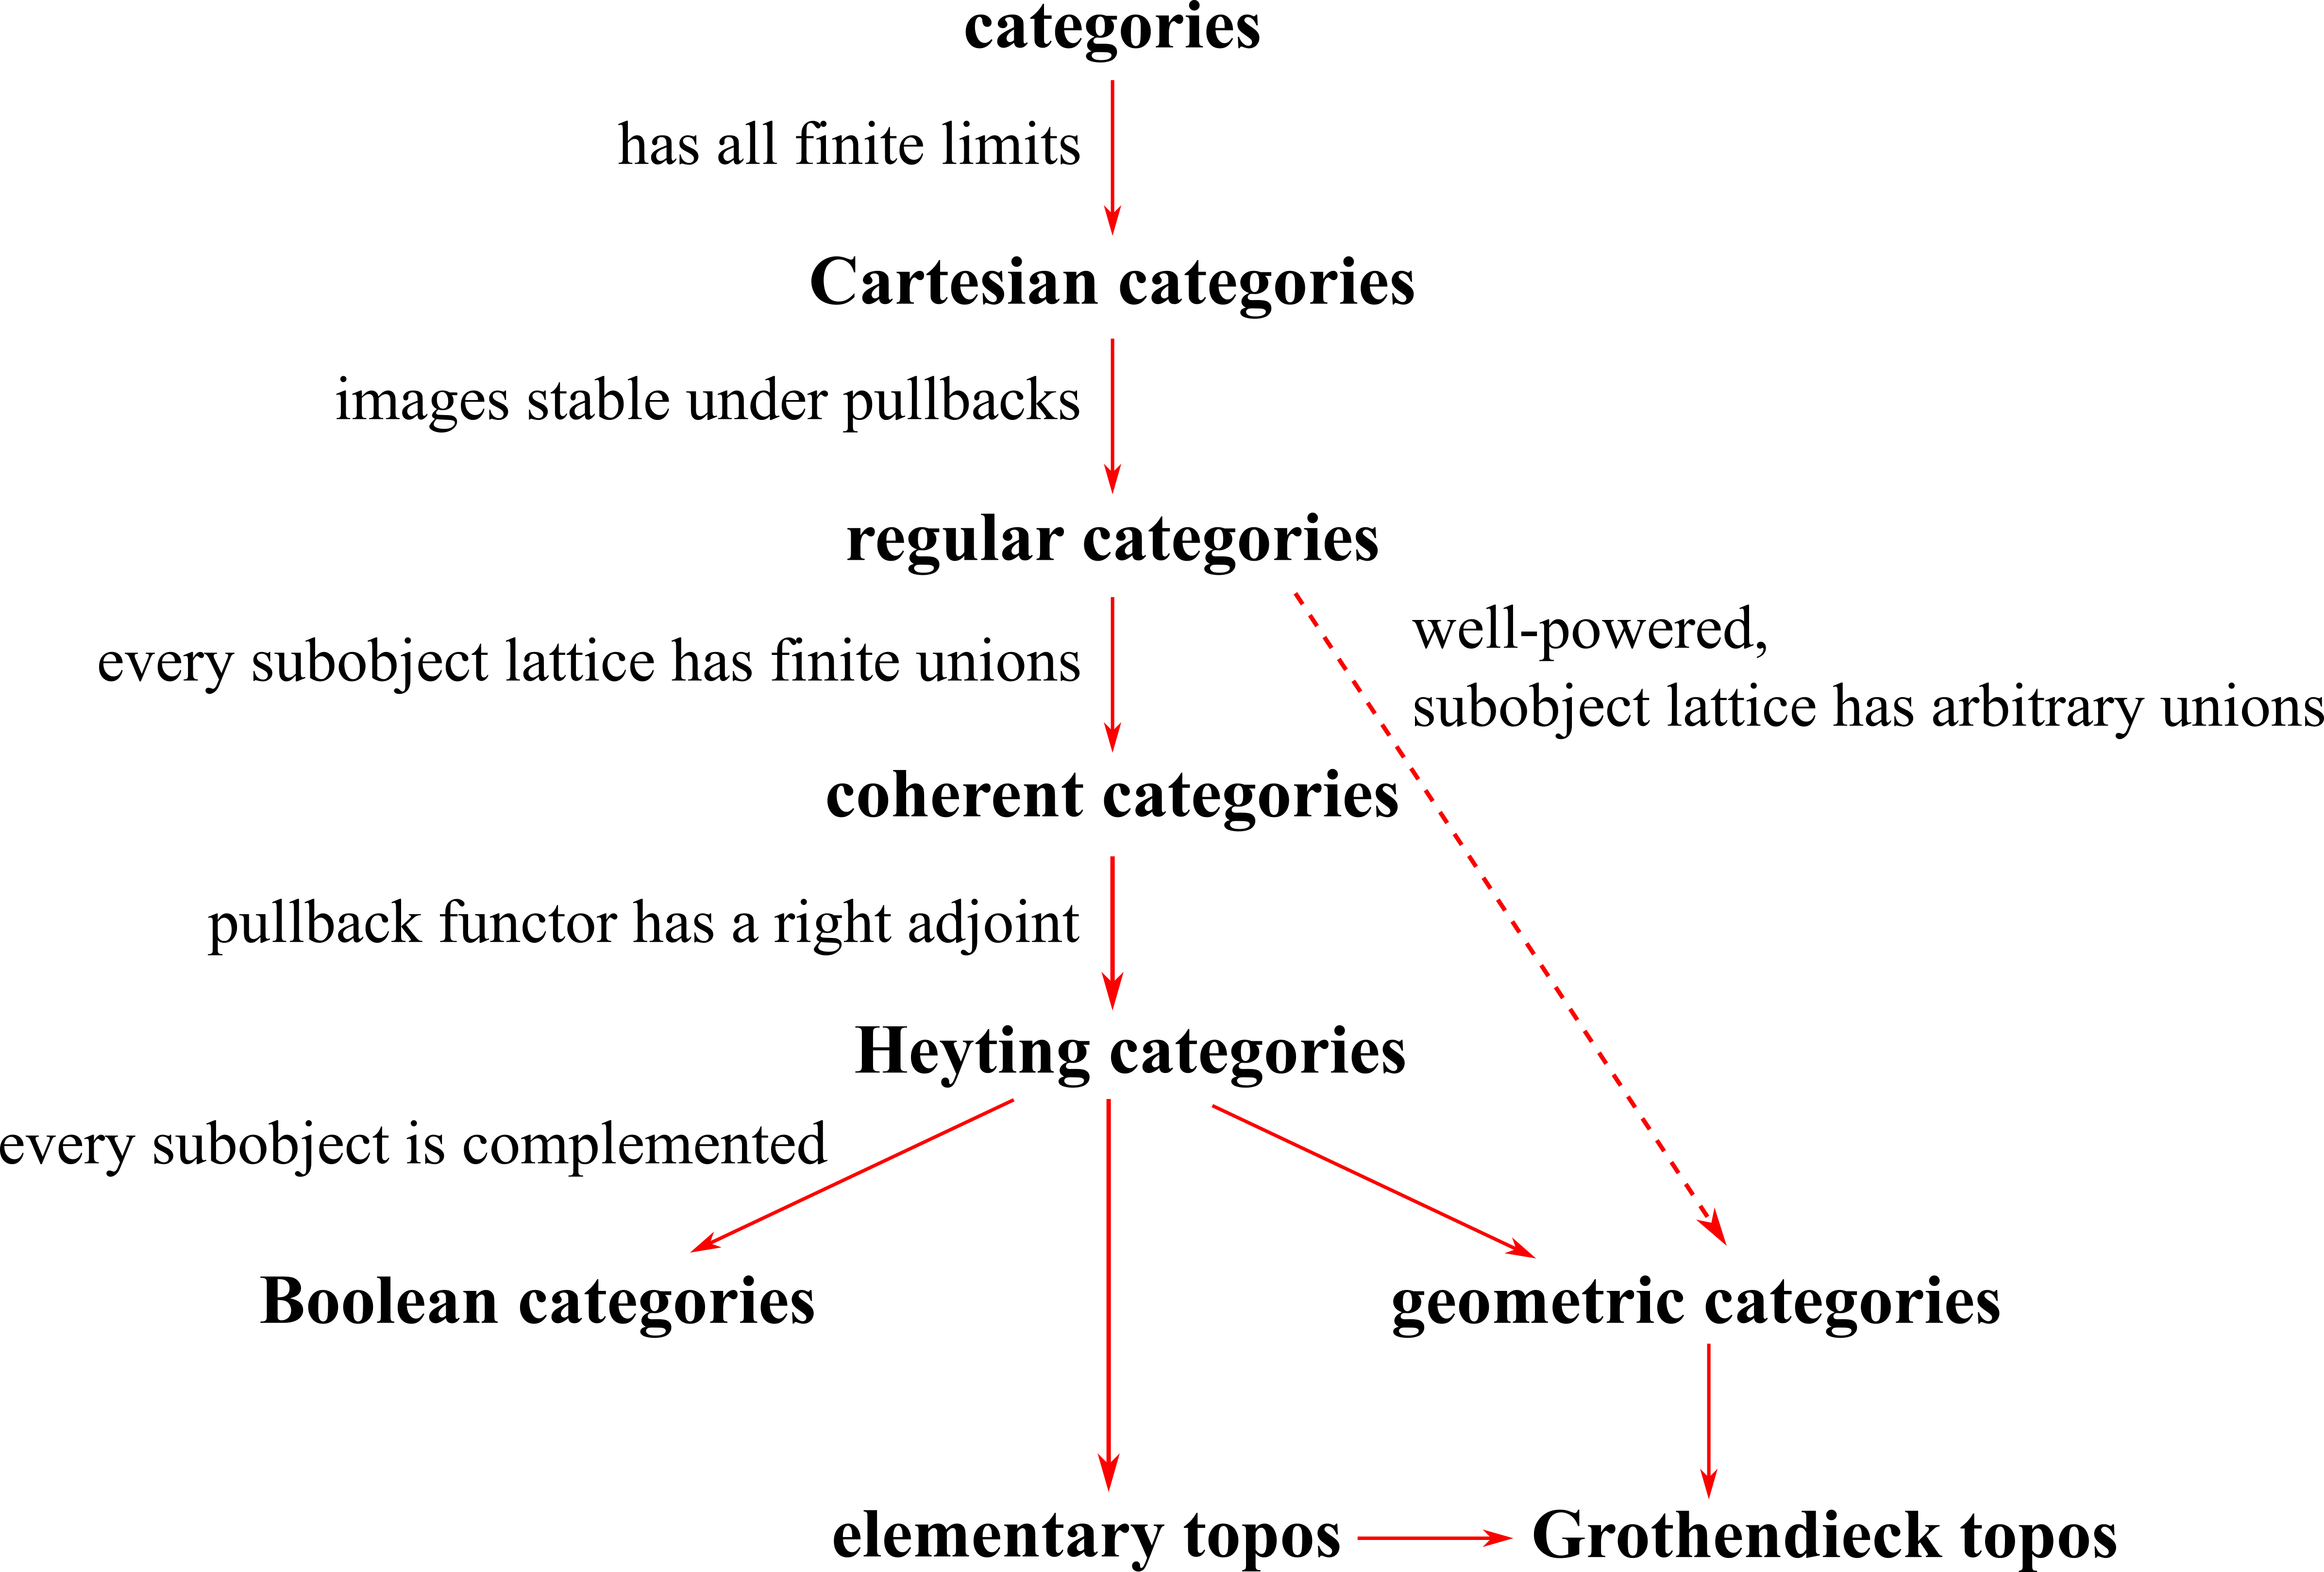
\includegraphics[scale=0.7]{logical-categories.png}}}
\end{equation}

\section{Domain theory}

$\lambda$-calculus 和 combinatory logic 都是可以表达任意 \textbf{函数} 的形式。 如果全体函数的 domain 是 $D$,而 由 $D \rightarrow D$ 的函数的个数是 $|D^D|$,则根据集合论的 Cantor's theorem,$|D^D|$ 必定大於 $|D|$,即使 $D$ 是无穷依然成立。 换句话说,$\lambda$-calculus 和 combinatory logic 不可能有 models。  这结论是非常令人不安的。 但在 1971 年,这个问题被 Dana Scott 和 C Strachey 解决了,开创了 \textbf{domain theory}。

以下内容主要来自 \parencite{Vickers1989},是一本很易懂的书,还有更新和更详尽的 \parencite{Goubault-Larrecq2013}.

Scott 的解决办法是给 domain $D$ \uline{endow with a \textbf{Scott topology},然后只考虑 $D \rightarrow D$ 的}\textbf{\uline{连续函数}}。 后者的数量较少,所以避开了 Cantor 勃论。 

..... 【未完待续】 $\NewSym{../UnderConst.png}$

\printbibliography

\end{document}